\documentclass[mathserif, aspectratio=169]{beamer}
\usetheme{odenpecos}
\setbeamertemplate{itemize/enumerate body begin}{\fontsize{8.8}{9}\selectfont}
\setbeamertemplate{itemize/enumerate subbody begin}{\fontsize{7.5}{8}\selectfont}
\setbeamertemplate{itemize/enumerate subsubbody begin}{\fontsize{7.5}{8}\selectfont}

% default search path for figures
\graphicspath{{./shared_figures/}{./figures/}}

\newcommand{\zapspace}{\topsep=0pt\partopsep=0pt\itemsep=0pt\parskip=0pt}

\usepackage{multicol}
\usepackage{pict2e}
\usepackage{esdiff}
\usepackage{multimedia}
\usepackage{verbatim}
\usepackage{mhchem}

\usepackage[percent]{overpic}
\usepackage[absolute,overlay]{textpos}

\newcommand{\overbar}[1]{\mkern 1.5mu\overline{\mkern-1.5mu#1\mkern-1.5mu}\mkern 1.5mu}
\newcommand{\pp}[2]{\frac{\partial #1}{\partial #2}}
\newcommand{\dd}[2]{\frac{d #1}{d #2}}
\newcommand{\DD}[2]{\frac{D #1}{D #2}}
\newcommand{\mm}{\mathbf{minmod}}
\def\etal{{\it et al~}}
\newcommand{\be}{\begin{eqnarray}}
\newcommand{\ee}{\end{eqnarray}}
\newcommand{\mbb}[1]{\mathbb{#1}} % math blackboard bold
\newcommand{\mcal}[1]{\mathcal{#1}} % math blackboard bold
\newcommand{\mbf}[1]{\mathbf{#1}} % math bold face (for vectors)
\newcommand{\sbf}[1]{\boldsymbol{#1}} % bold face for symbols
\newcommand{\jump}[1]{\llbracket #1 \rrbracket} % jump operator
\newcommand{\avg}[1]{\langle #1 \rangle} % average operator
\newcommand{\rarrow}{\rightarrow}
\newcommand{\Rarrow}{\Rightarrow}
\newcommand{\LRarrow}{\Leftrightarrow}
\newcommand{\vvvert}{|\kern-1pt|\kern-1pt|}
\newcommand{\enorm}[1]{\vvvert #1 \vvvert}
\newcommand{\nutil}{\tilde{\nu}}
\newcommand{\Var}{\mathrm{Var}}
\newcommand{\Cov}{\mathrm{Cov}}


\definecolor{MyDarkGreen}{rgb}{0,0.45,0.08}
\newcommand{\myred}[1]{{\color{red} #1}}
\newcommand{\myblue}[1]{{\color{blue} #1}}
\newcommand{\mygreen}[1]{{\color{MyDarkGreen} #1}}

\newcommand{\sa}{\nu_{\mathrm{sa}}}
\newcommand{\tep}{\tilde{\epsilon}}
\newcommand{\Ssd}{\mathcal{S}} % source term due to slow derivative
\newcommand{\ud}{\,\mathrm{d}}

\newcommand{\Mach}[1]{\ensuremath{\mbox{Ma}_{#1}}}
\newcommand{\Reynolds}{\ensuremath{\mathit{Re}}}
\newcommand{\DensityRat}{\ensuremath{\mathit{DR}}}
\newcommand{\BlowRat}{\ensuremath{\mbox{BR}}}
\newcommand{\VelRat}{\ensuremath{\mathit{VR}}}
\newcommand{\Tau}{\ensuremath{\mathrm{T}}}

\newcommand{\wall}     {\ensuremath{\mathrm{w}}}   % wall subindex
\newcommand{\awall}    {\ensuremath{\mathrm{aw}}}  % adiabatic wall subindex

\newcommand{\commentout}[1]{}

\newcommand{\vect}[1]{\boldsymbol{#1}}
\usepackage{mleftright}
\newcommand{\of}[1]{\mleft( #1 \mright)}
\newcommand{\vth}{v_{\textrm{th}}}
\newcommand{\reals}{\mathbb{R}}
\newcommand{\myint}{\int\limits}
\newcommand{\ddt}[1]{\partial_t #1}
\newcommand{\RR}{\mathbb{R}}
\newcommand{\vr}{v}
%\newcommand{\vtheta}{\theta_{\vect{v}}}
%\newcommand{\vphi}{\varphi_{\vect{v}}}
%\newcommand{\vr}{v_{r}}
\newcommand{\vtheta}{v_{\theta}}
\newcommand{\vphi}{v_{\varphi}}
\newcommand{\vomega}{v_{\omega}}
\newcommand{\vrunit}{\hat{\vect{v}}_{r}}
\newcommand{\vthetaunit}{\hat{\vect{v}}_{\theta}}
\newcommand{\vphiunit}{\hat{\vect{v}}_{\varphi}}
\DeclareMathOperator{\variance}{Var}

\begin{document}
% disable nav
\setbeamertemplate{navigation symbols}{}

% ---------------------------------------------------------------
% Oden/Pecos title page

%\hoffset=.16in
%
%\begin{frame}[plain,t]{}
%\makeatletter
%%\vspace*{0.85cm}
%%\vspace*{0.65cm}
%\includegraphics[height=0.9in,trim=50 40 40 0, clip]{PMSc_159_university_formal_horizontal.pdf} \newline
%%\vspace*{0.3cm}
%\begin{columns}[T,onlytextwidth]
%\column{.8\textwidth}
%{\bf \color{burntorange} \fontfamily{bch}\selectfont 
%% -- Set talk title here
%Solving the Boltzmann equation for electron kinetics using Petrov-Galerkin approach
%% --
%}
%\end{columns}
%\vspace*{.15cm}
%\rule{.8\textwidth}{0.6pt} \newline
%
%\vspace*{0.05cm}
%\setstretch{0.65}
%{\fontfamily{phv}\selectfont
%  { \scriptsize
%    % -- define presenter, authors here
%    Milinda Fernando, Daniil Bochkov, Todd Oliver, George Biros\newline
%    % --
%  }
%  {\color{burntorange} \tiny
%    % -- define role, meeting event, location, etc
%    Year-1 Review $\cdot$ August, 2021 $\cdot$ Austin, TX
%    % --
%  }
%}
%
%\vspace*{1cm}
%%\includegraphics[height=0.3in]{figures/pecos_orange1.png}
%\begin{columns}
%\begin{column}{0.8\linewidth}
%\includegraphics[height=0.5in]{oden_pecos_2020_wordmark.png}\\
%{\scriptsize \url{https://pecos.oden.utexas.edu}}
%\end{column}
%
%\begin{column}{0.2\linewidth}
%\includegraphics[height=0.6in]{psaap3-logo.png}
%\end{column}
%\end{columns}
%
%\end{frame}
%\hoffset=0in
% -- end title slide ---------------------------------------------

\begin{frame}{Collision operator with corrected basis}
	\begin{columns}
		\begin{column}{0.5\textwidth}
			Maxwell polynomials
			\small
			\begin{align*}
				\Phi_{klm} (\vect{v}) &= \exp\left(-\left(\frac{v_r}{v_{th}}\right) ^ 2\right)  P_{kl}\of{\frac{v_r}{v_{th}}} Y_{lm}(v_\theta,v_\phi) \\
				\Psi_{pqs} (\vect{v}) &= P_{pq}\of{\frac{v_r}{v_{th}}} Y_{qs}(v_\theta,v_\phi)
			\end{align*}
			\begin{itemize}
				\item Mass matrix is orthonomal.  
			\end{itemize}
		\end{column}
		\begin{column}{0.5\textwidth}
			B-Splines 
			\small
			\begin{align*}
			\Phi_{klm} (\vect{v}) &= \left(\frac{v_r}{v_{th}}\right)^l P_k\of{\frac{v_r}{v_{th}}} Y_{lm}(v_\theta,v_\phi) \\
			\Psi_{pqs} (\vect{v}) &= \left(\frac{v_r}{v_{th}}\right)^q P_p\of{\frac{v_r}{v_{th}}} Y_{qs}(v_\theta,v_\phi)
			\end{align*}
			\begin{itemize}
				\item ill-conditioning of the mass matrix treated with pseudo inverse. 
				\item knots are placed in log scale
				\item pseudo inverse allows placing knots closer to $v=0$
			\end{itemize}
		\end{column}
	\end{columns}
\end{frame}

%\begin{frame}
%\frametitle{Discretized collision kernel with Maxwell (T=3eV) singular values}
%\begin{table}
%	\centering
%	\begin{tabular}{cc}
%		$l_{max}=0$ &  $l_{max}=1$ \\
%		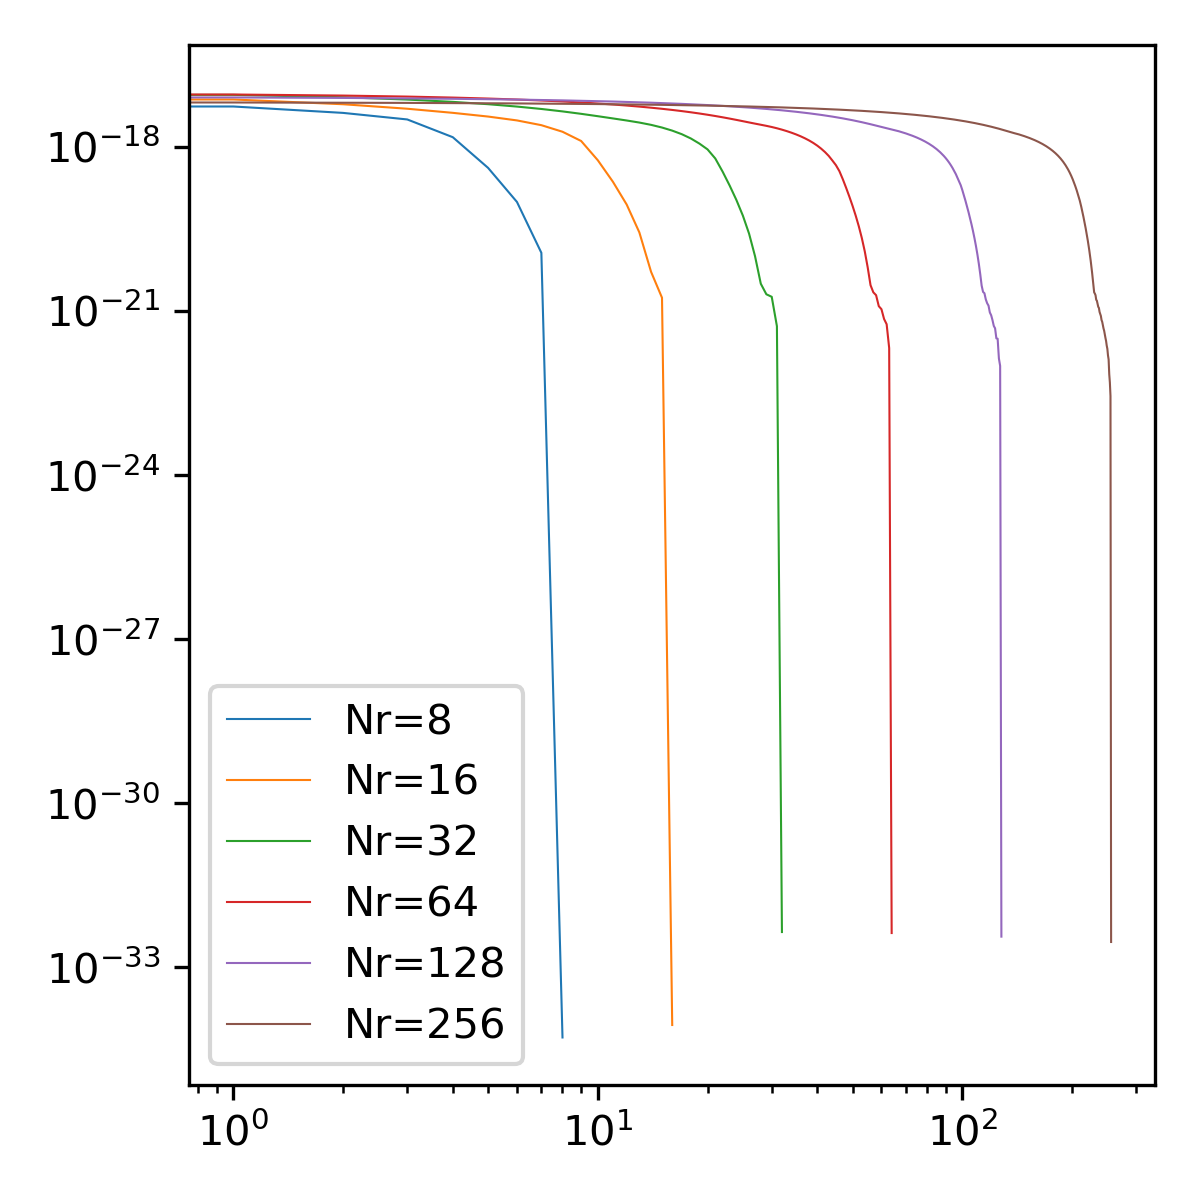
\includegraphics[width=0.3\textwidth]{figures/m_spectrum_3ev_l_max_0.png} & 
%		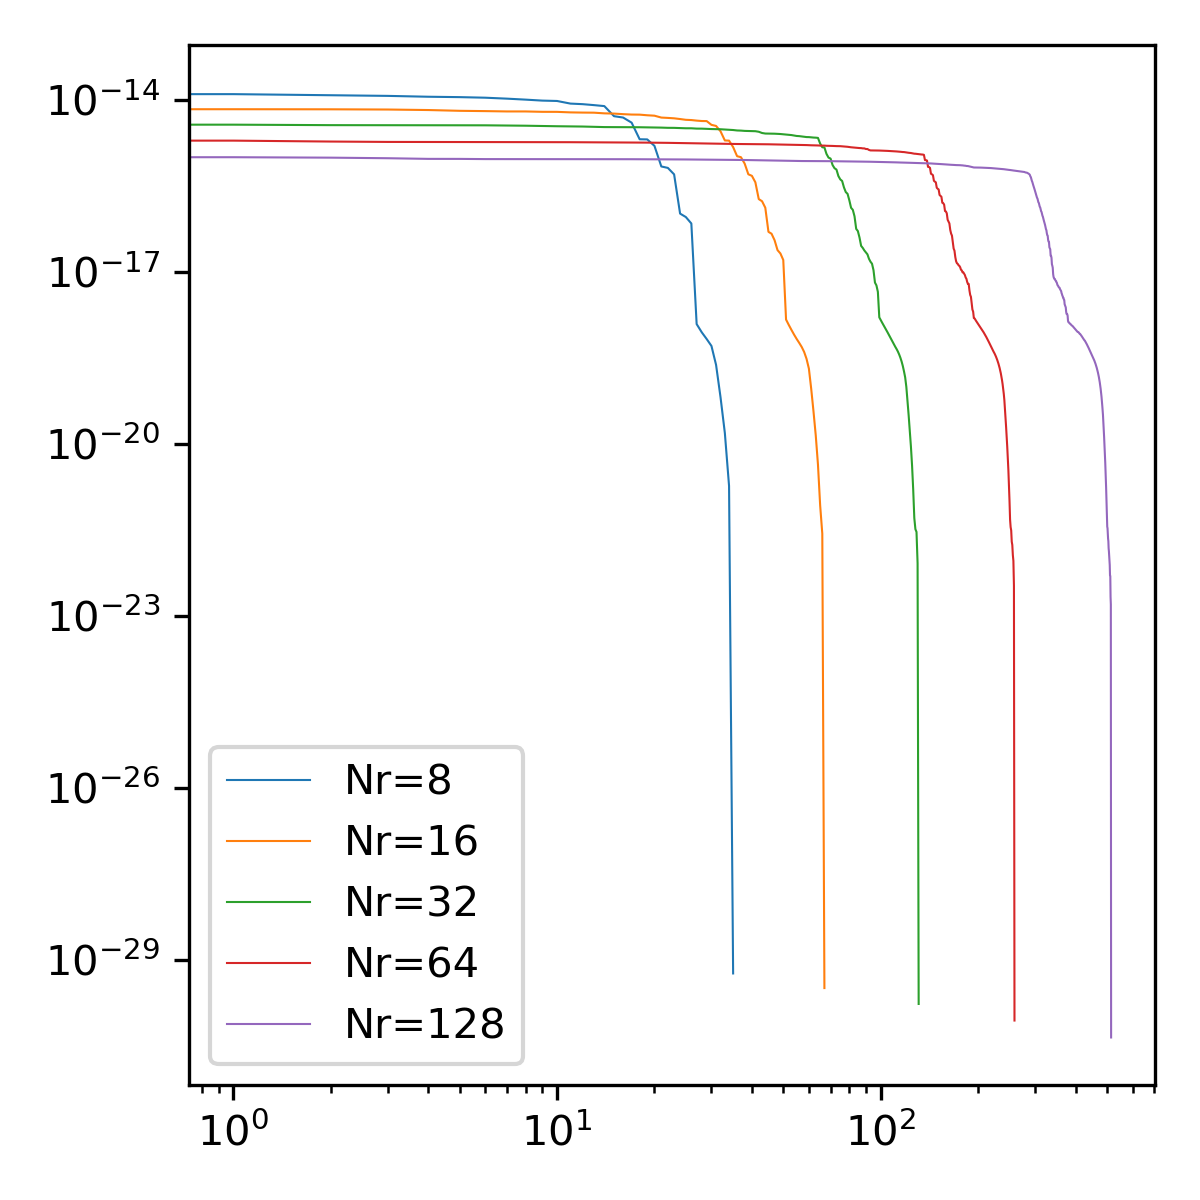
\includegraphics[width=0.3\textwidth]{figures/m_spectrum_3ev_l_max_1.png} 
%	\end{tabular}
%\end{table}
%Currently the differential cross section is uniform across all scattering angles. 
%\end{frame}


\begin{frame}
	\frametitle{Discretized collision kernel singular values}
	\only<+>{
	\begin{table}
		\centering
		\begin{tabular}{cc}
			Maxwell &  linear splines \\
			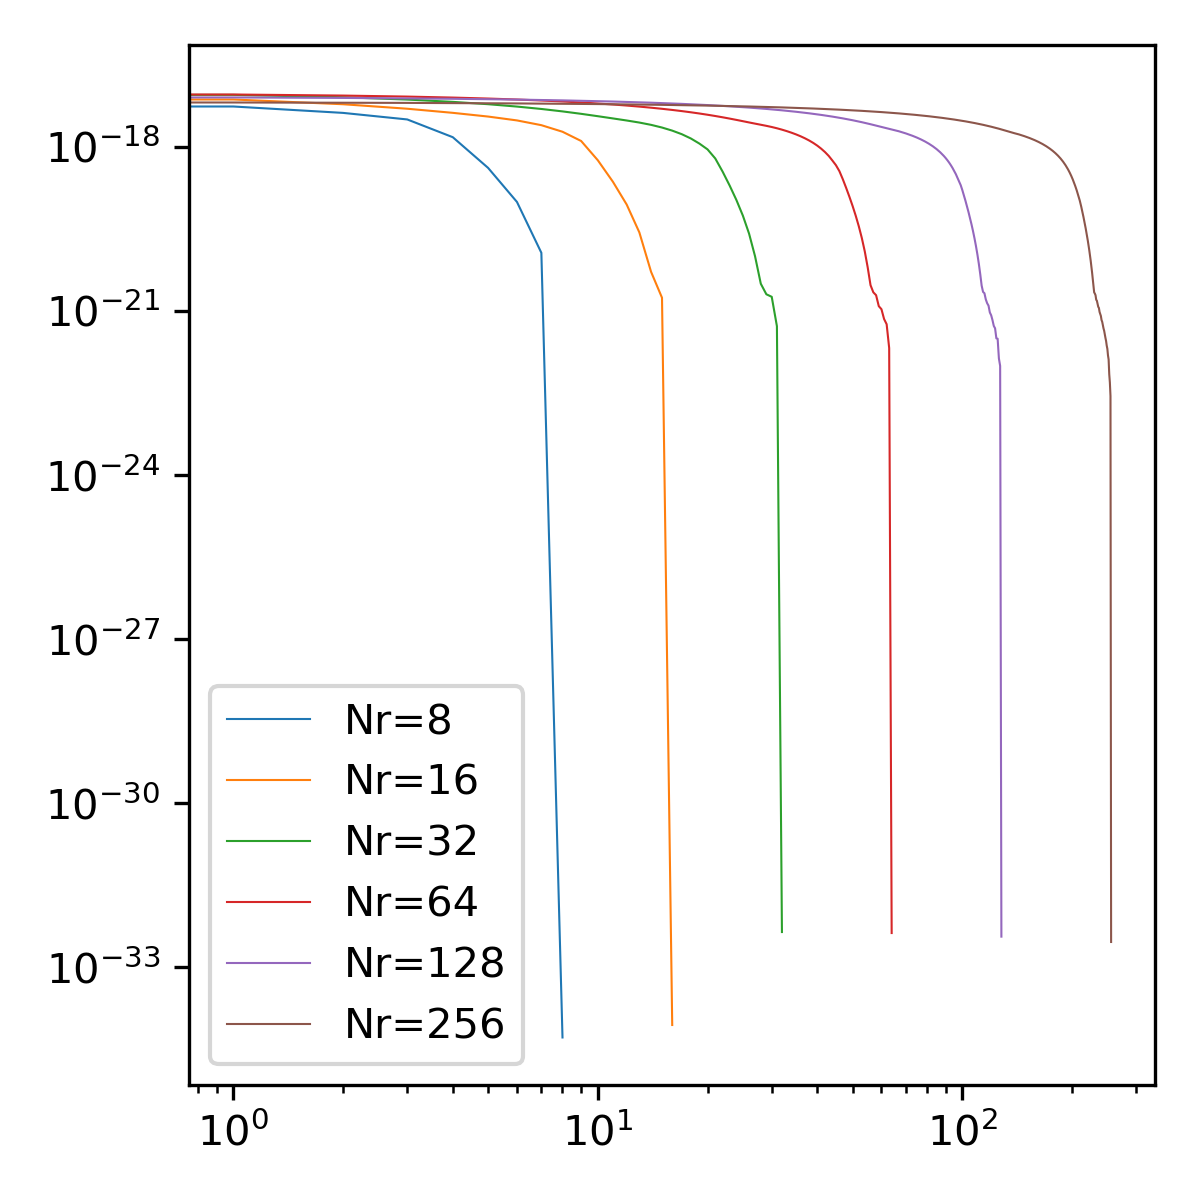
\includegraphics[width=0.35\textwidth]{figures/m_spectrum_3ev_l_max_0.png} & 
			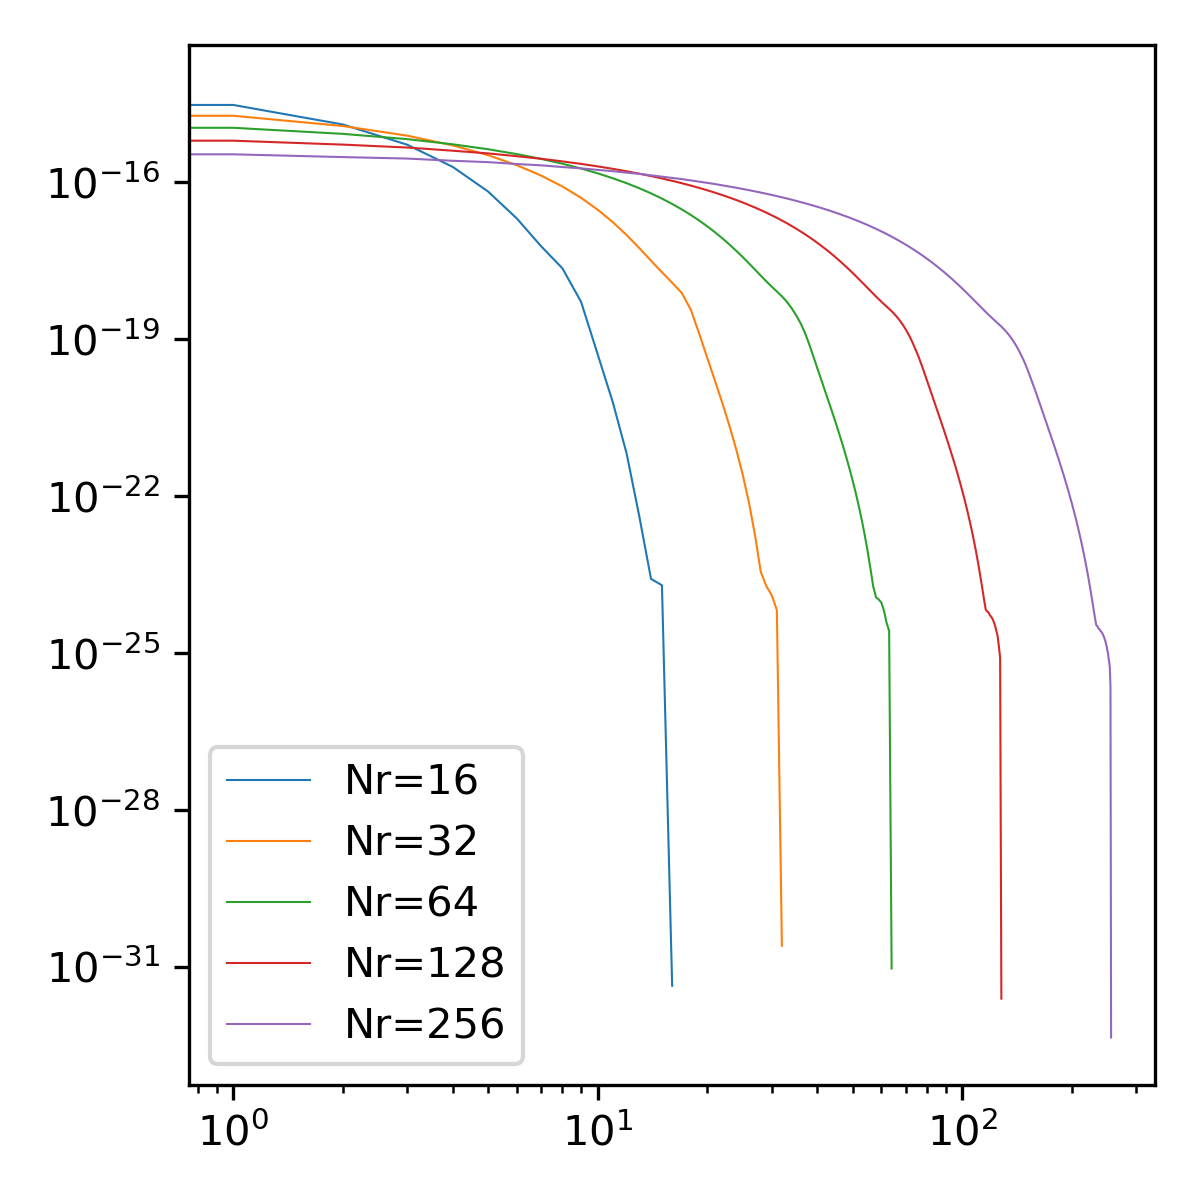
\includegraphics[width=0.35\textwidth]{figures/b_sp1_spectrum_3ev_l_max_0.png} 
		\end{tabular}
	\end{table}}
%	\only<+>{
%	\begin{table}
%		\centering
%		\begin{tabular}{cc}
%			Maxwell &  quadratic splines \\
%			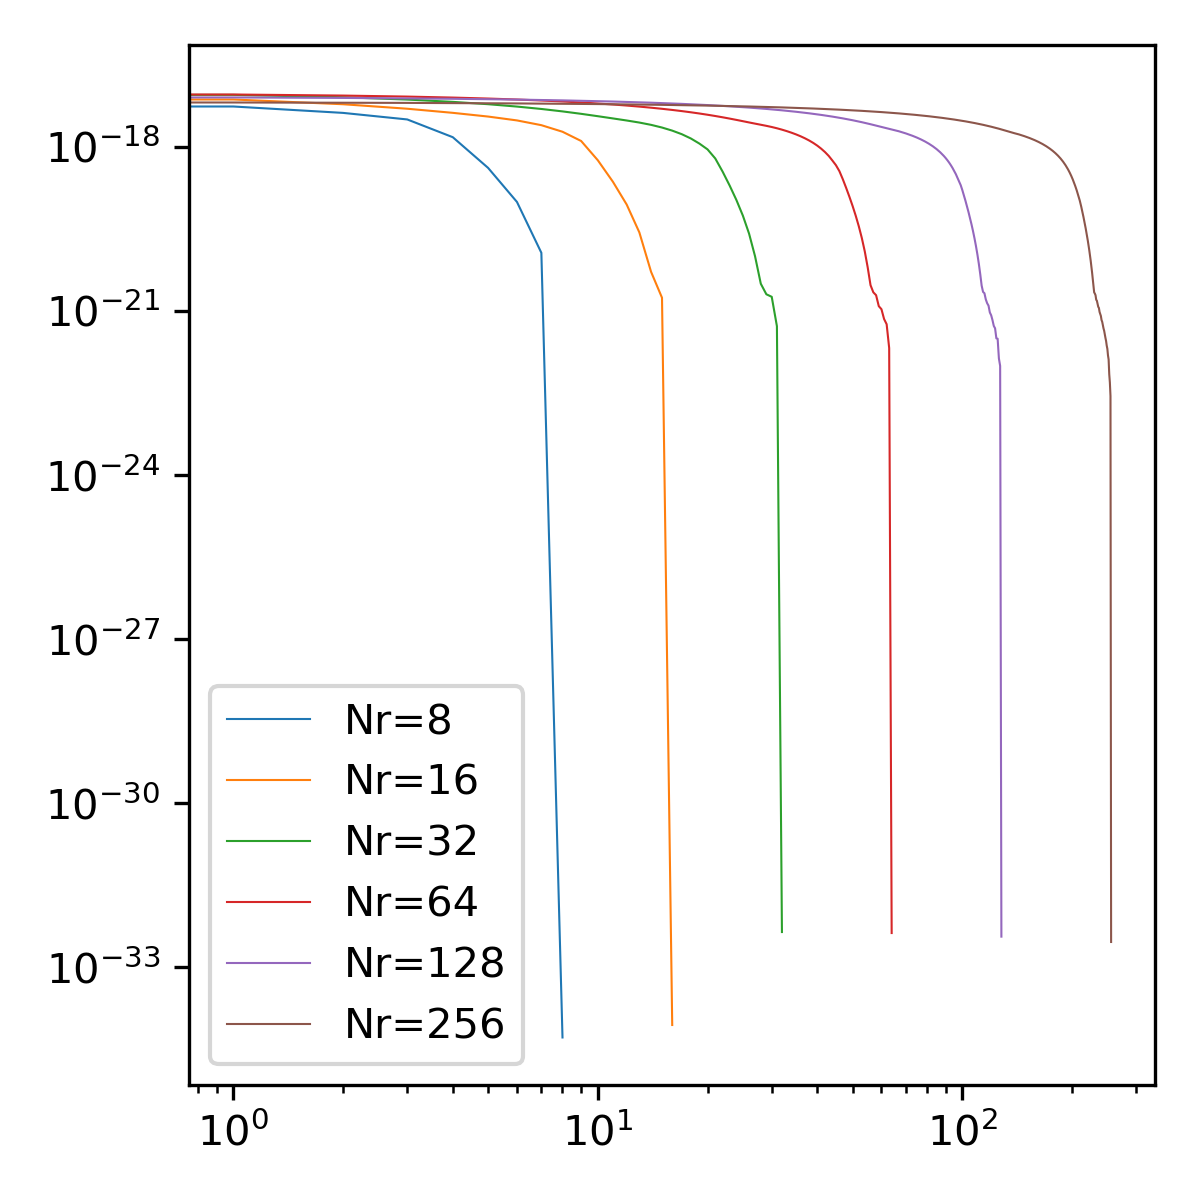
\includegraphics[width=0.35\textwidth]{figures/m_spectrum_3ev_l_max_0.png} & 
%			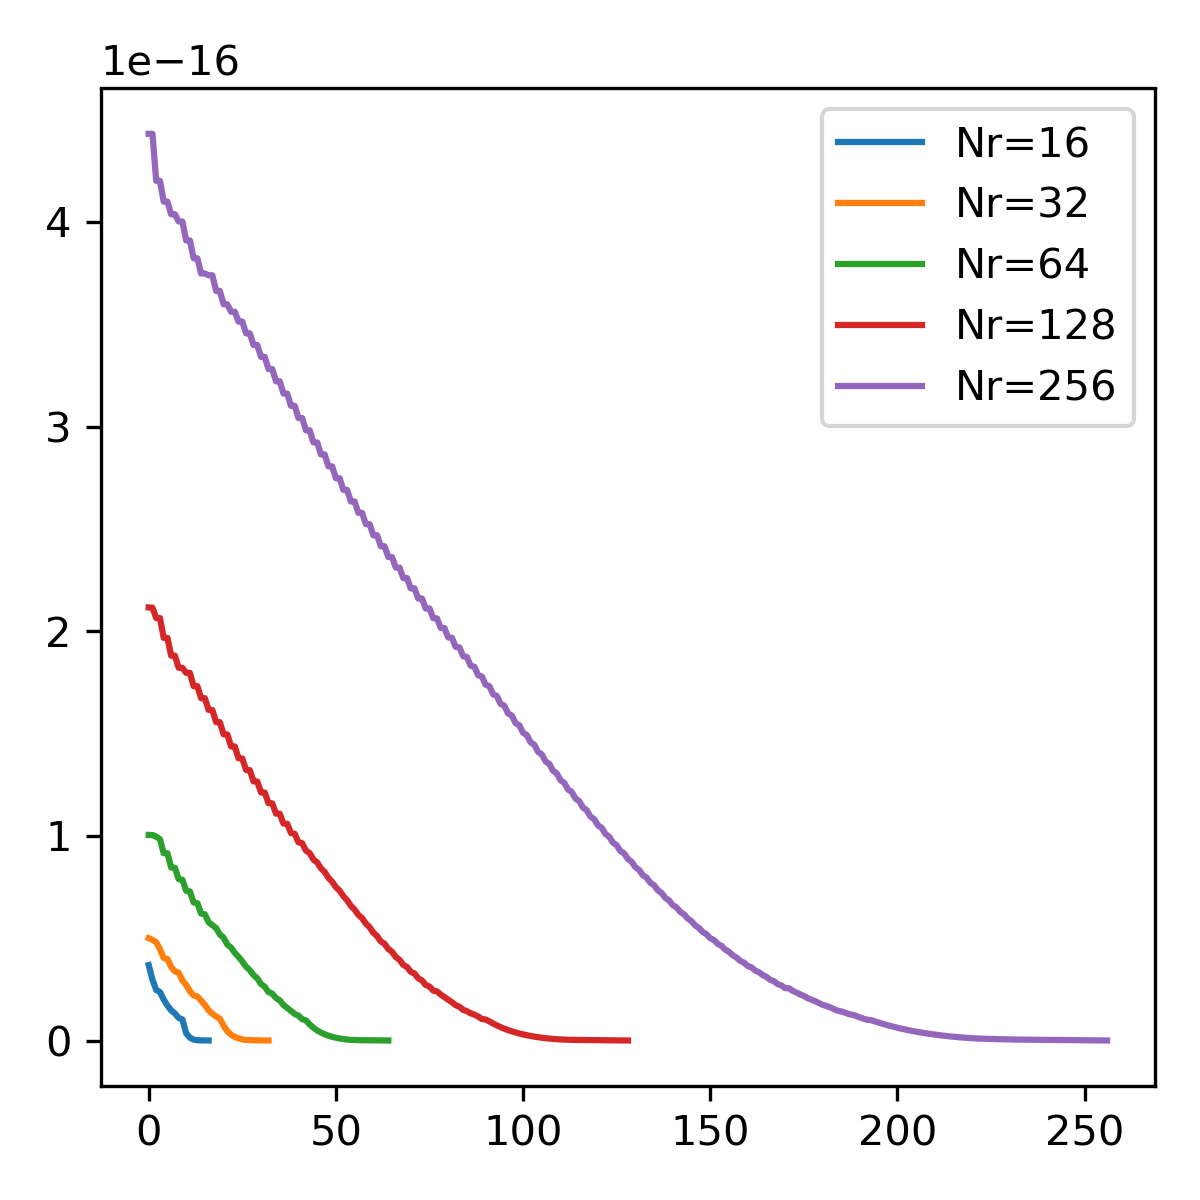
\includegraphics[width=0.35\textwidth]{figures/b_sp2_spectrum_3ev_l_max_0.png} 
%		\end{tabular}
%\end{table}}
%	\only<+>{
%	\begin{table}
%		\centering
%		\begin{tabular}{cc}
%			Maxwell &  cubic splines \\
%			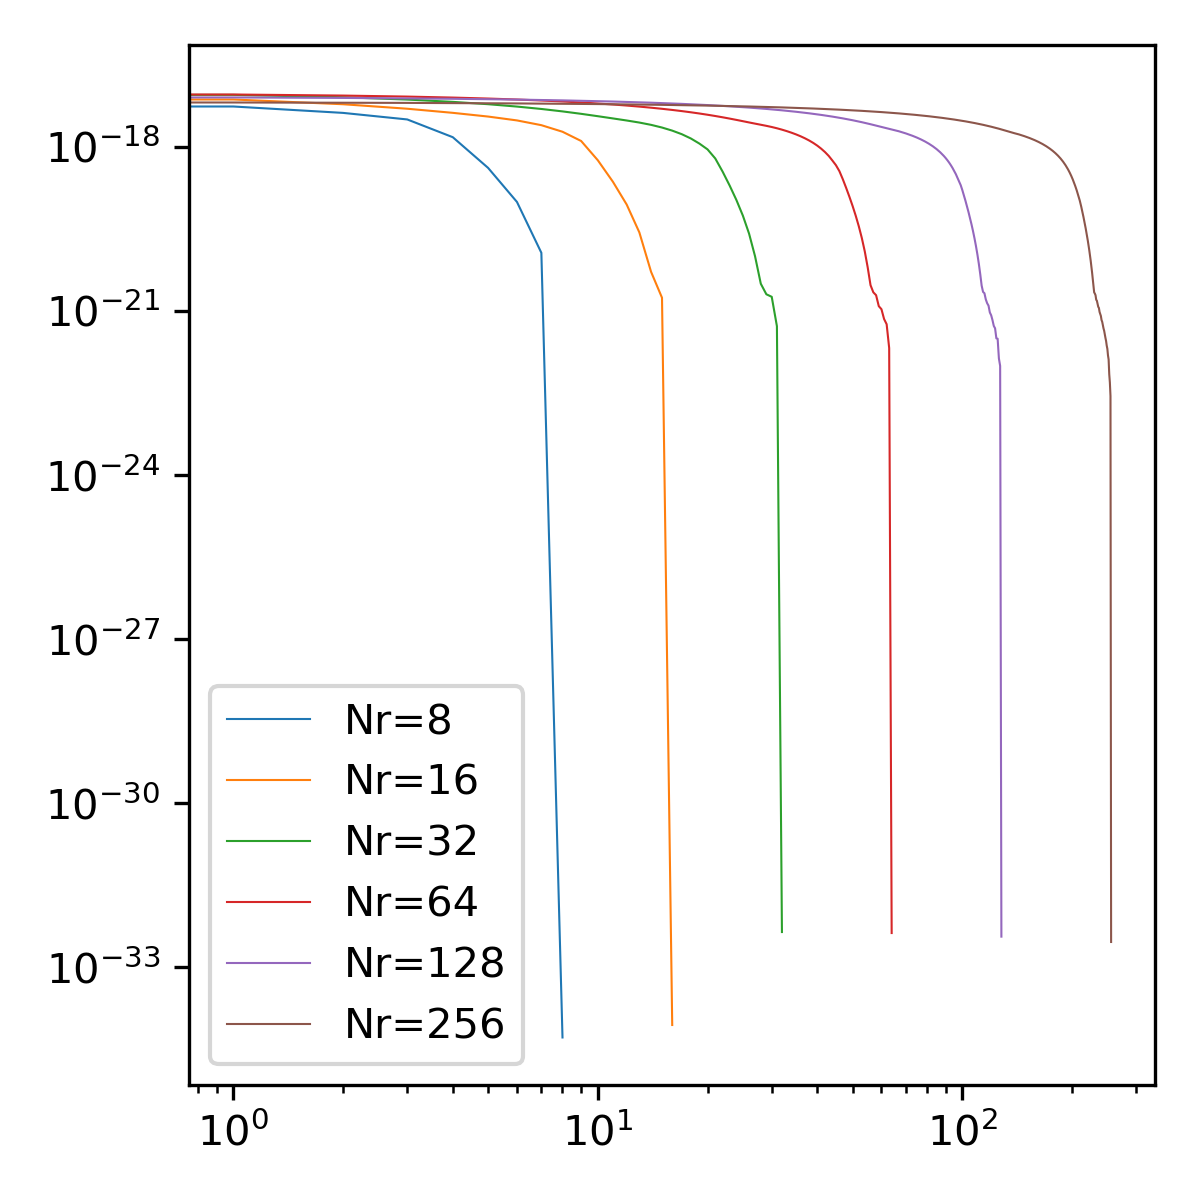
\includegraphics[width=0.35\textwidth]{figures/m_spectrum_3ev_l_max_0.png} & 
%			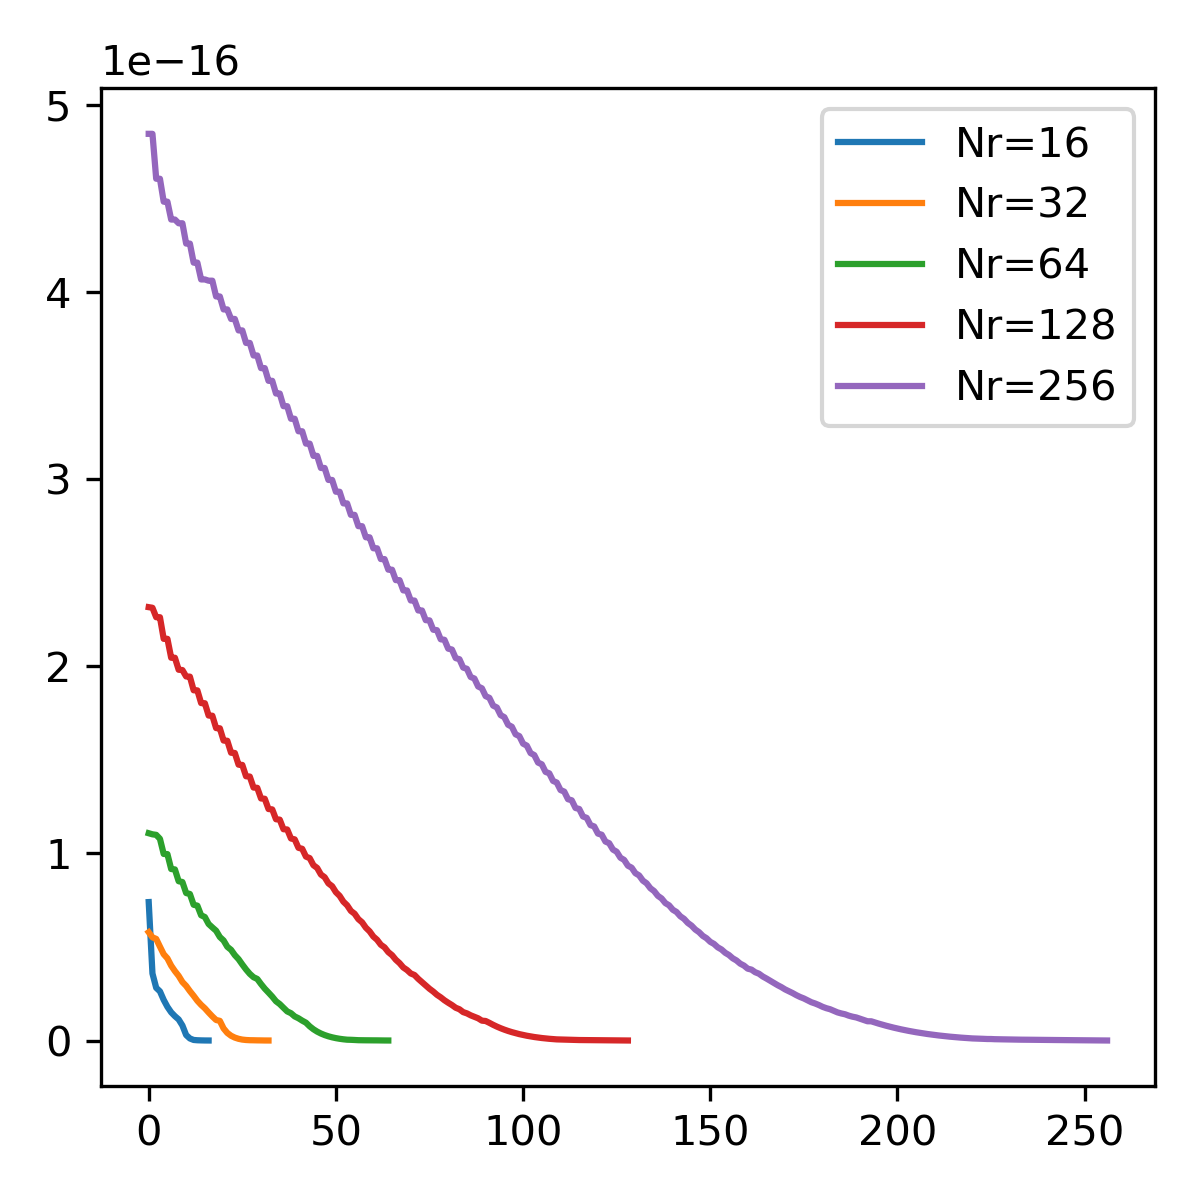
\includegraphics[width=0.35\textwidth]{figures/b_sp3_spectrum_3ev_l_max_0.png} 
%\end{tabular}
%\end{table}}
\begin{itemize}
	\item Difference between $max(\sigma)$ can be due to the norm differences between the projection operators.
\end{itemize}
\end{frame}

\begin{frame}
	\frametitle{B-Splines projection}
	\begin{itemize}
		\item Mass matrix for splines is ill-conditioned. 
		\item Using Cholesky factorization based inversion has improved the projection coefficient accuracy for b-splines. 
	\end{itemize}
\begin{table}
	\centering
	\begin{tabular}{cc}
		svd pseudo-inverse $\sigma_{c} = 10^{-15}\max\sigma$ &  Cholesky factored inverse \\
		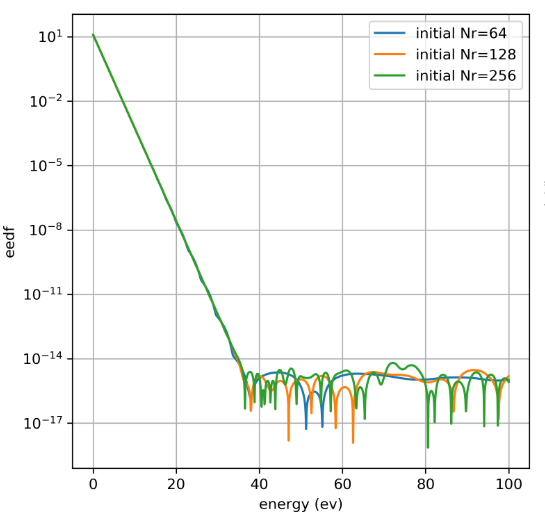
\includegraphics[width=0.35\textwidth]{figures/svd_pseudo_inv.png} &
		\includegraphics[width=0.35\textwidth]{figures/cholesky_inv.png} 
	\end{tabular}
\end{table}
\end{frame}


\begin{frame}
\frametitle{Elastic + Ionization at 1eV : Maxwell}
\begin{figure}
	\centering
	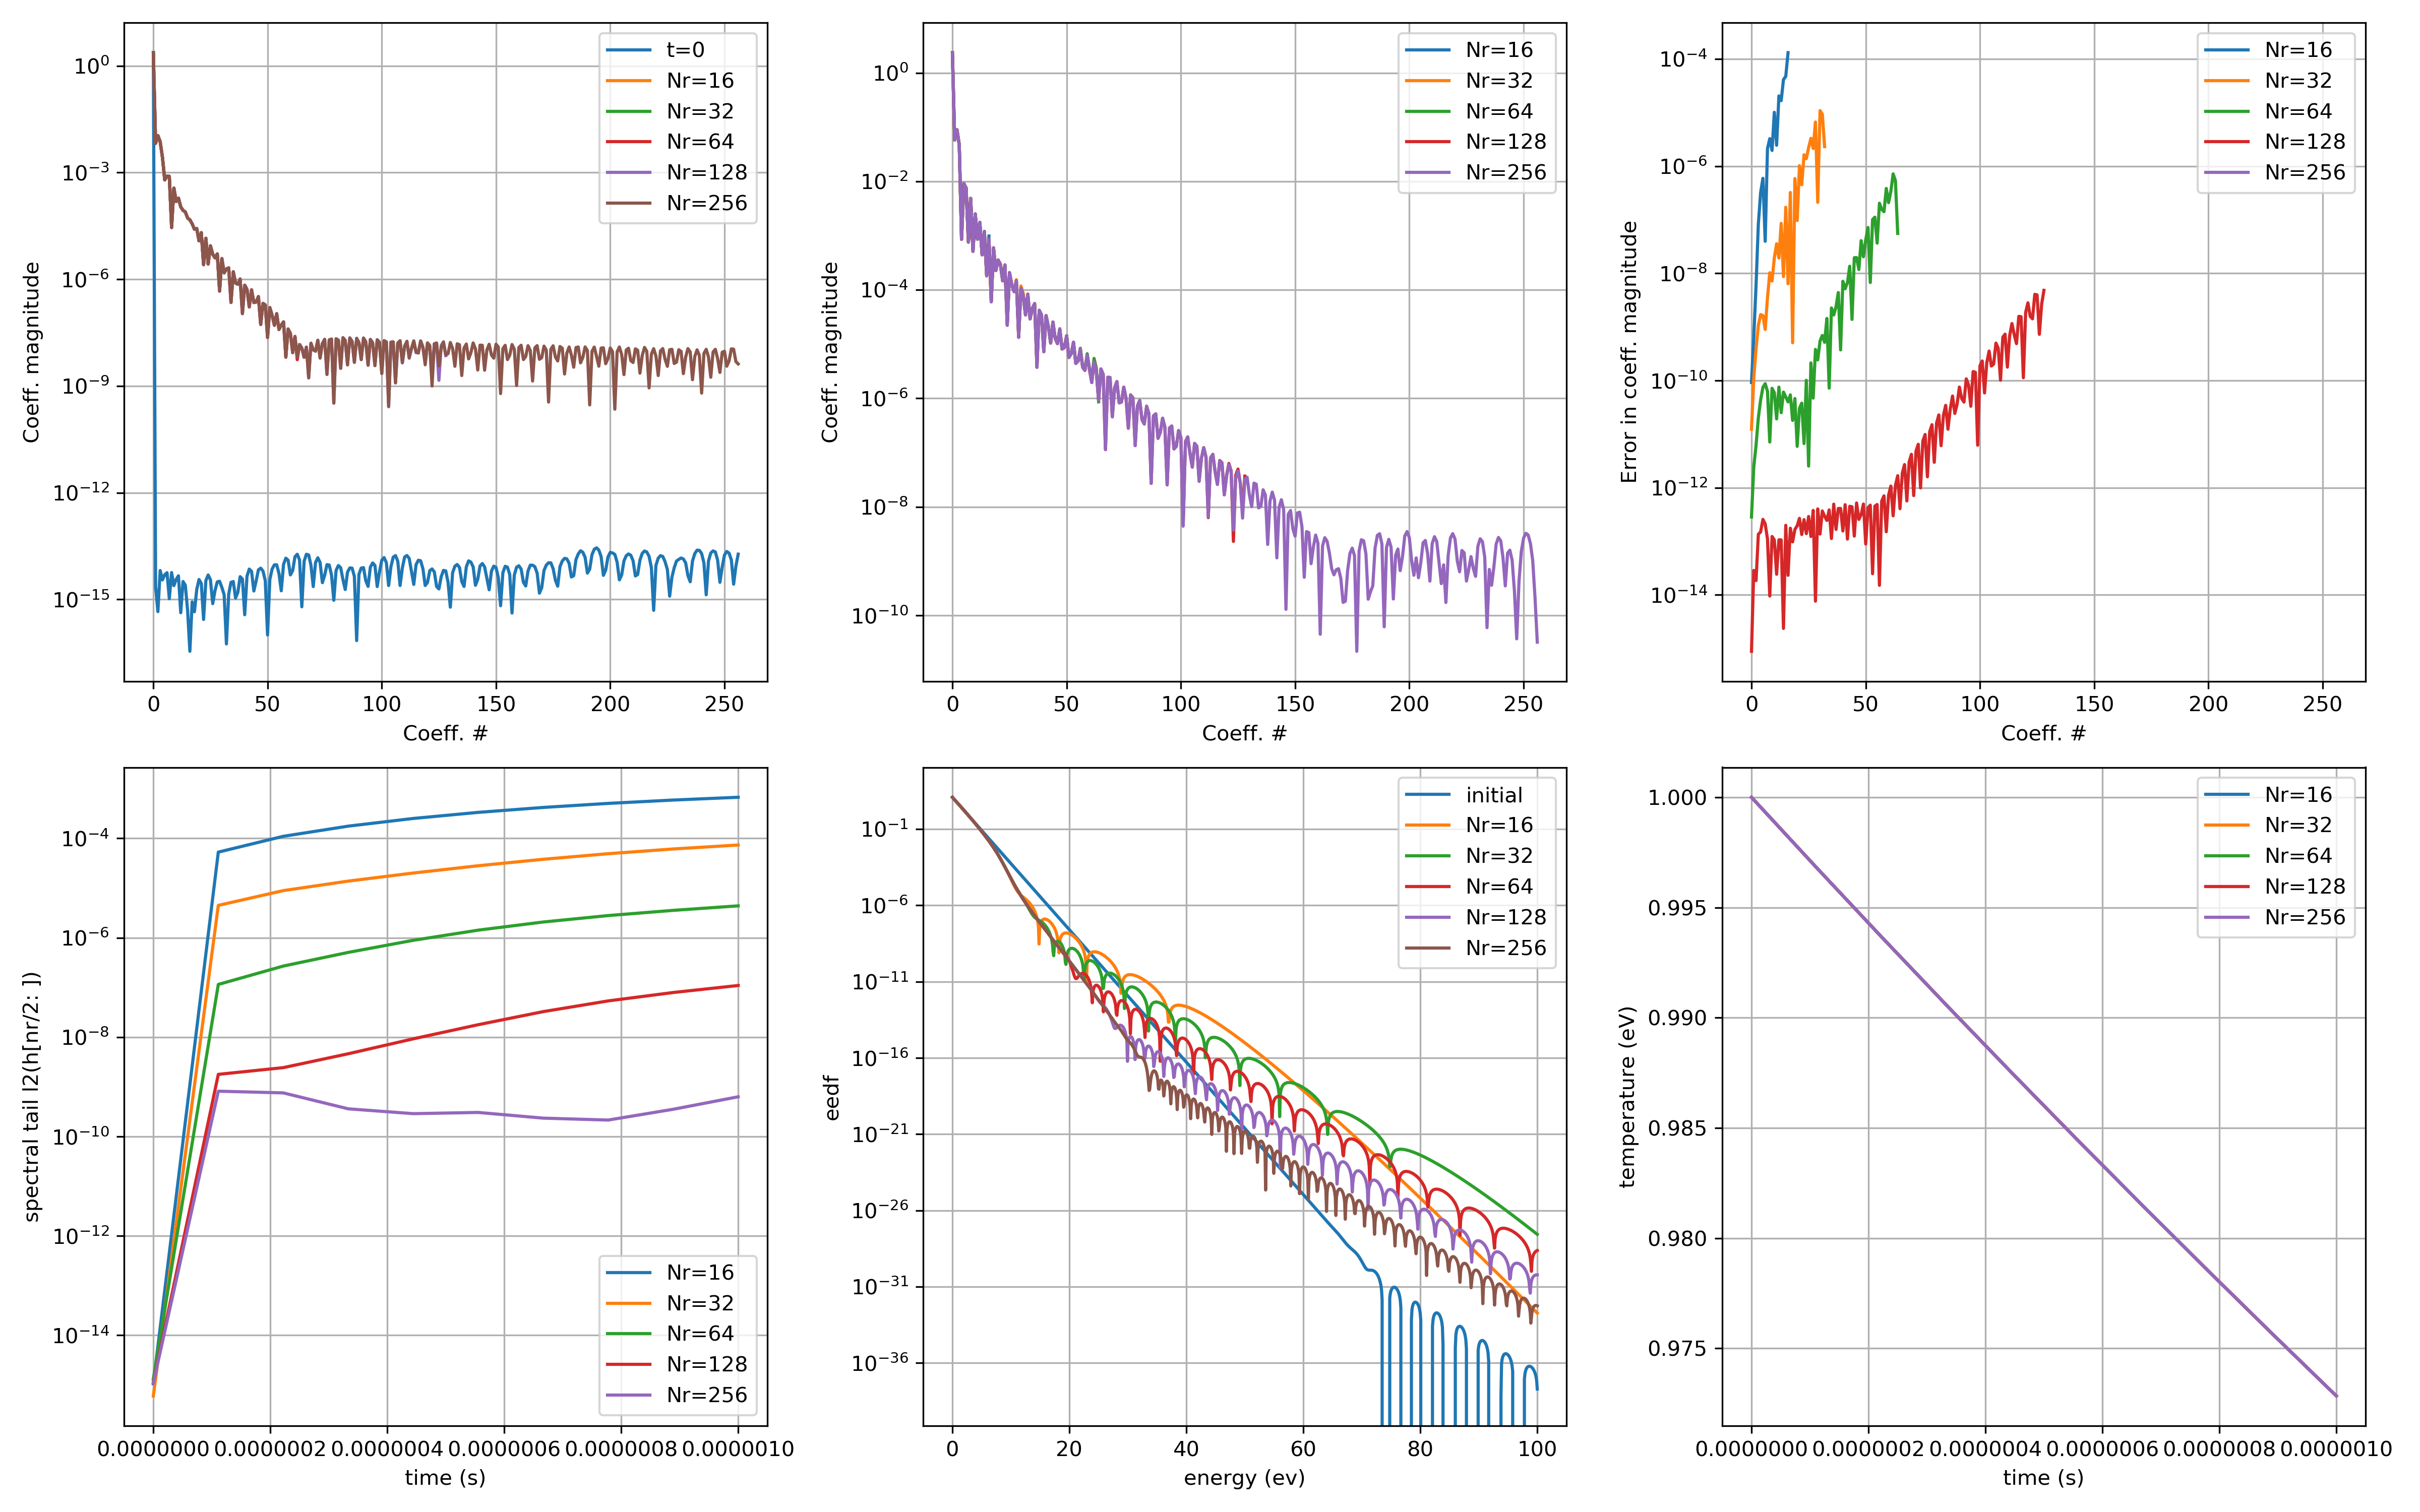
\includegraphics[width=0.7\textwidth]{figures/m_1ev_coeff.png}
\end{figure}
\end{frame}

\begin{frame}
	\frametitle{Elastic + Ionization at 1eV : Linear splines}
	\begin{figure}
		\centering
		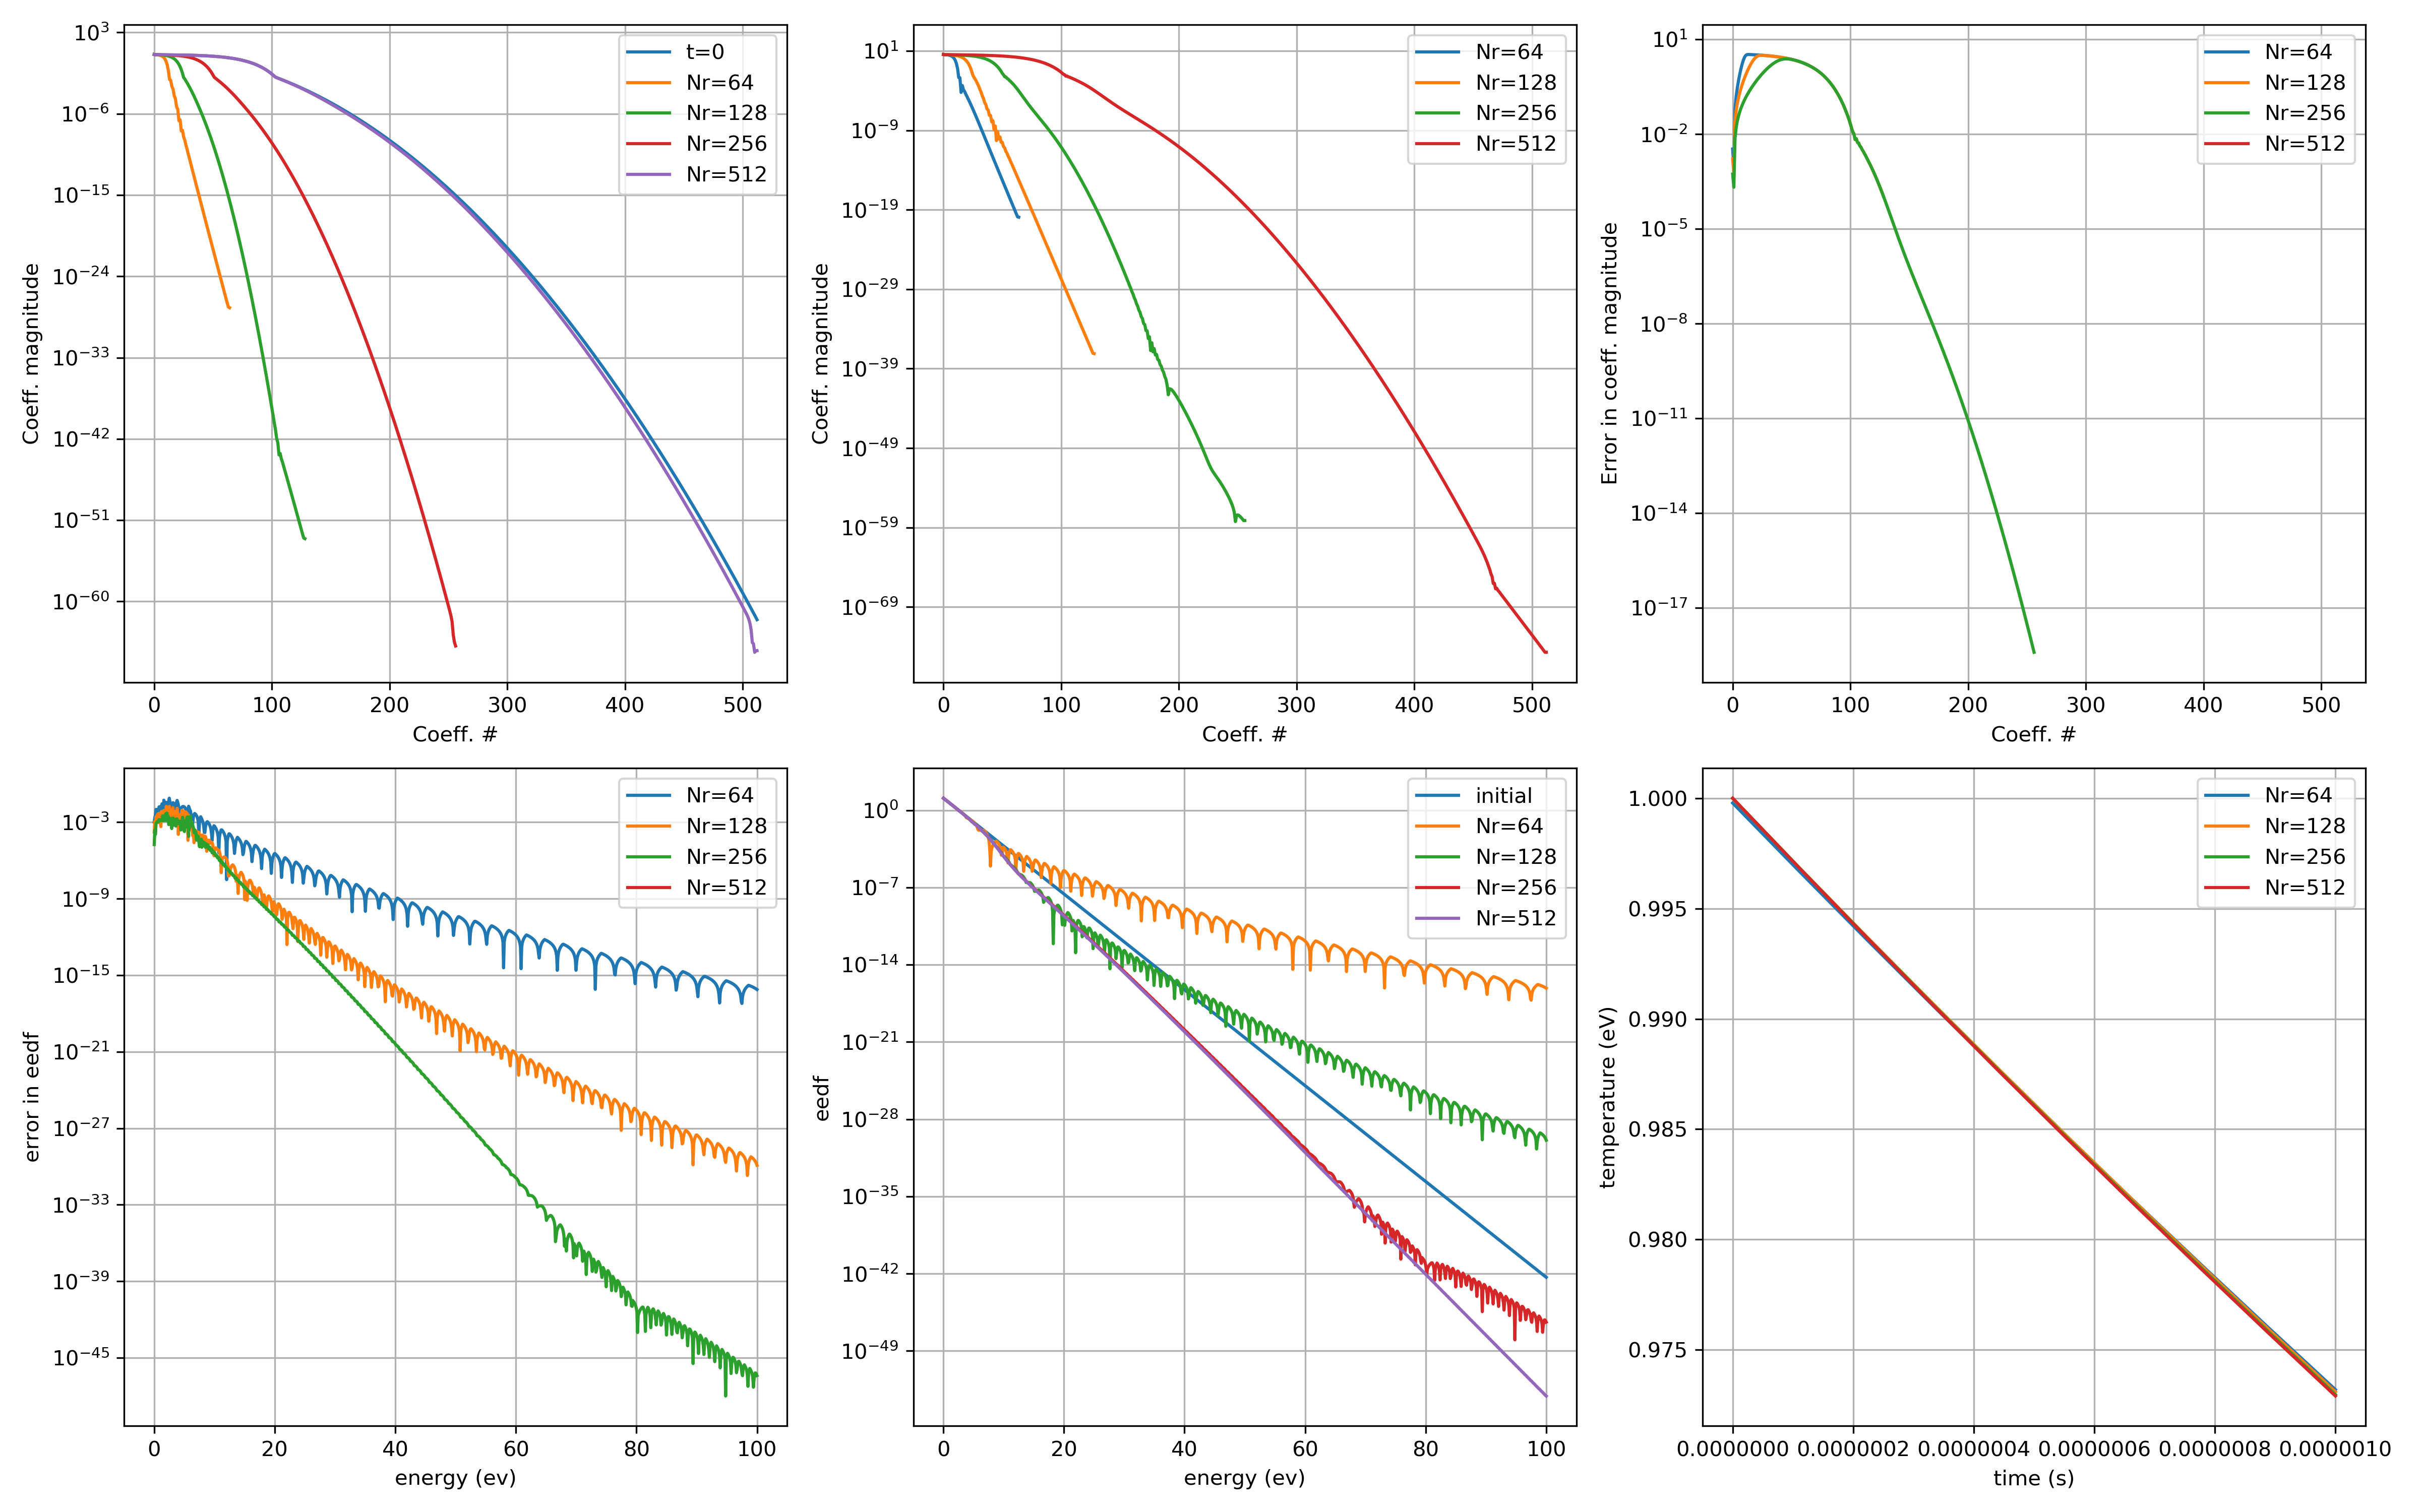
\includegraphics[width=0.7\textwidth]{figures/b_1ev_coeff.png}
	\end{figure}
\end{frame}


\begin{frame}
	\frametitle{Accuracy tests}
	With elastic collisions without energy transfer and with angle independent differential cross section, isotropic distribution should stay isotropic during evolution. We start with $f(\vect{v},t=0) = M(\vect{v})$
	
	\begin{table}
		\centering
		\begin{tabular}{cc}
			Maxwell &   linear splines\\
			\includegraphics[width=0.45\textwidth]{figures/m_1ev_no_cooling_coeff.png} & 
			\includegraphics[width=0.45\textwidth]{figures/b_1ev_no_cooling_coeff.png} 
		\end{tabular}
	\end{table}
\end{frame}

\begin{frame}
	\frametitle{Accuracy tests}
	With elastic collisions without energy transfer and with angle independent differential cross section, if we start with anisotropic distribution we should reach isotropic distribution eventually. We start with $f(\vect{v},t=0) = M(\vect{v}) (1 + \tan v_\theta)$, evolved for time horizon T=4e-6 s.
	\begin{figure}
		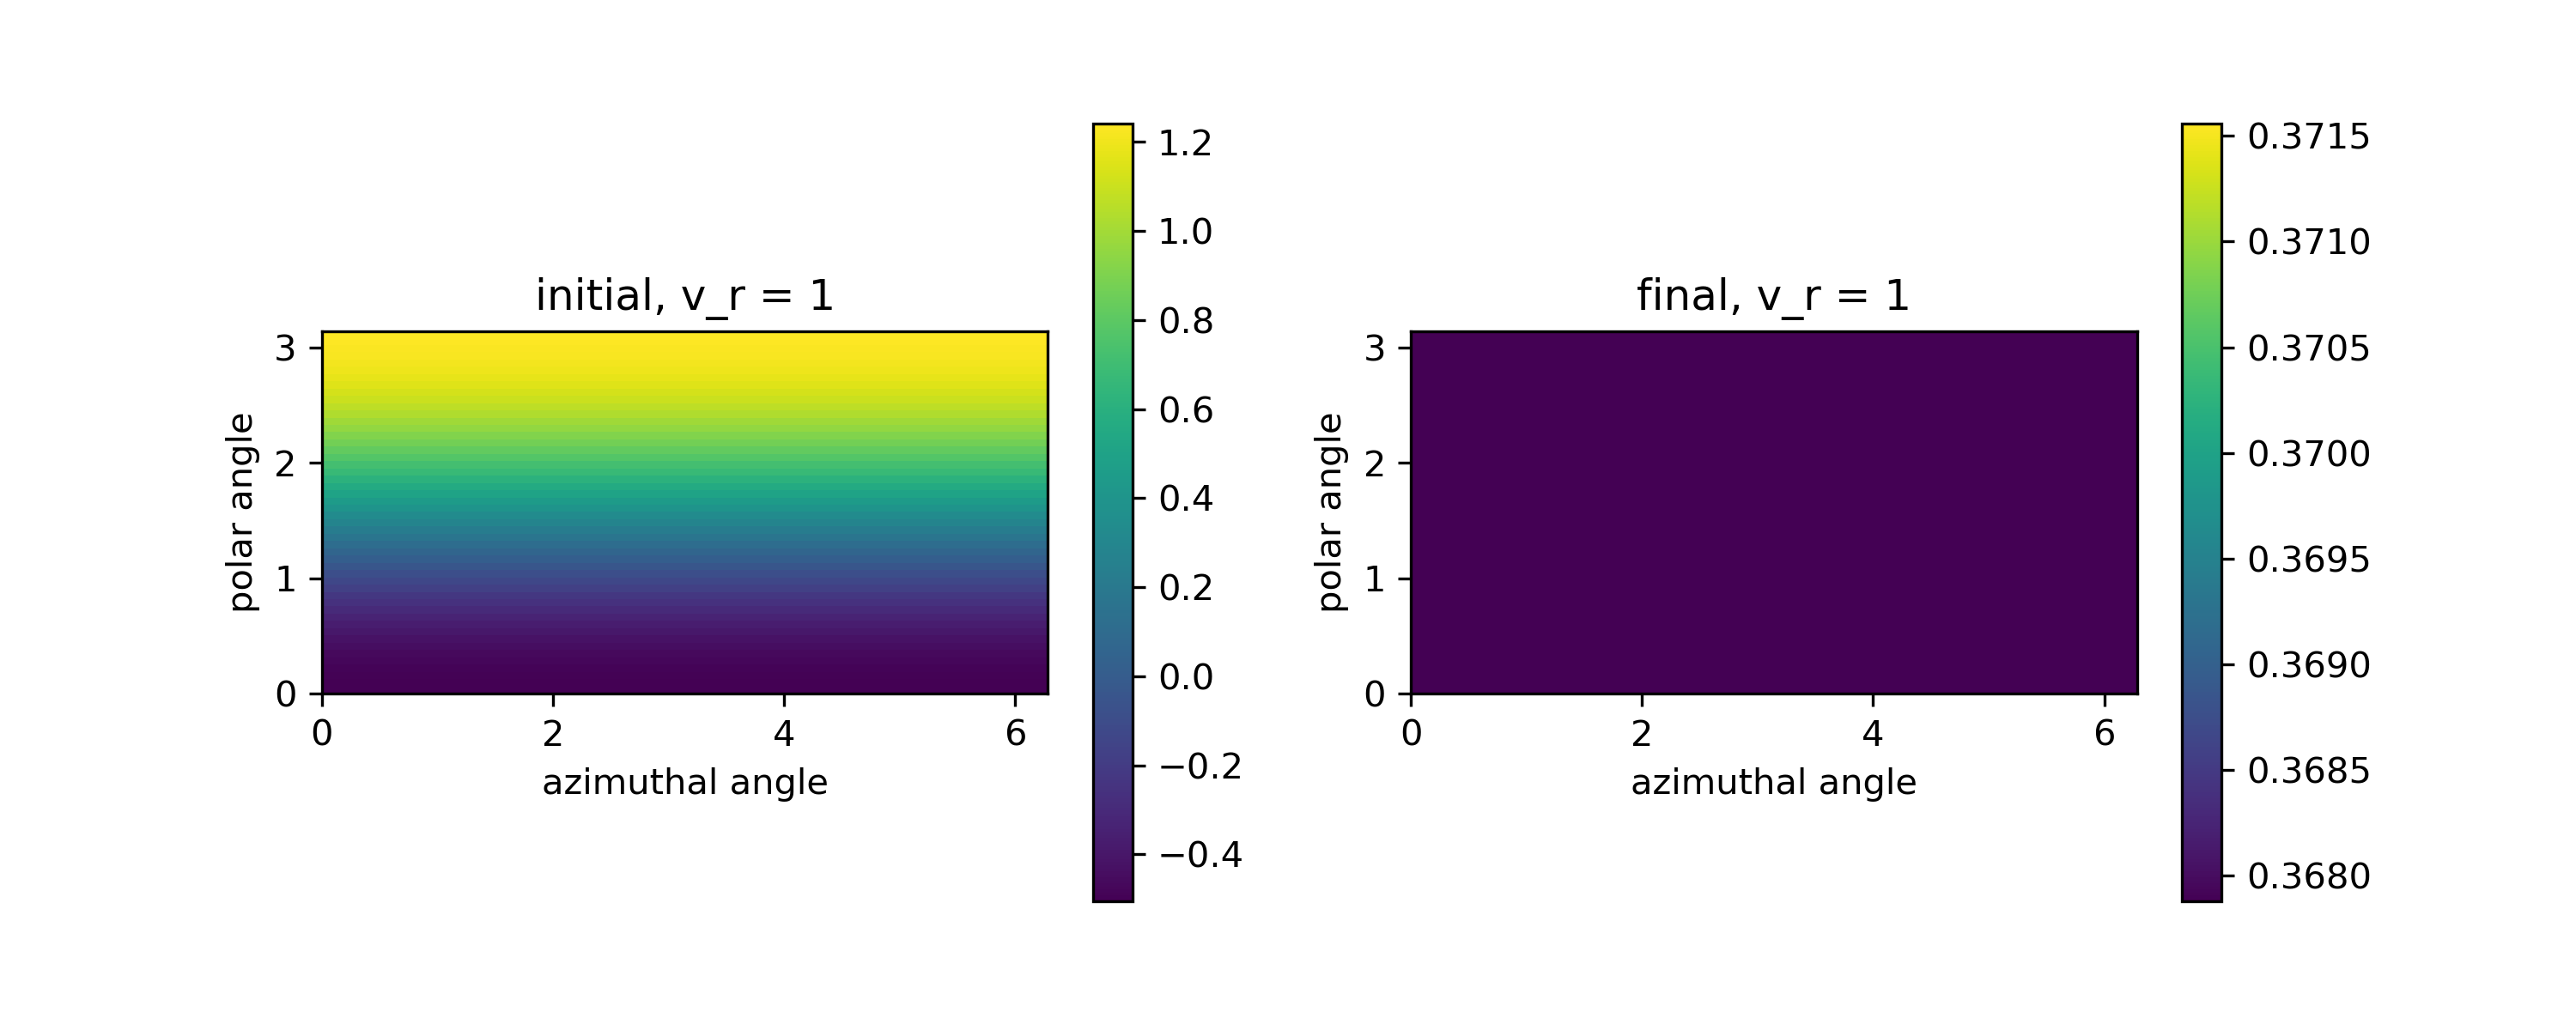
\includegraphics[width=0.48\textwidth]{figures/m_no_e_loss_aiso_test_1ev_4e-6_l2_const_r.png}
		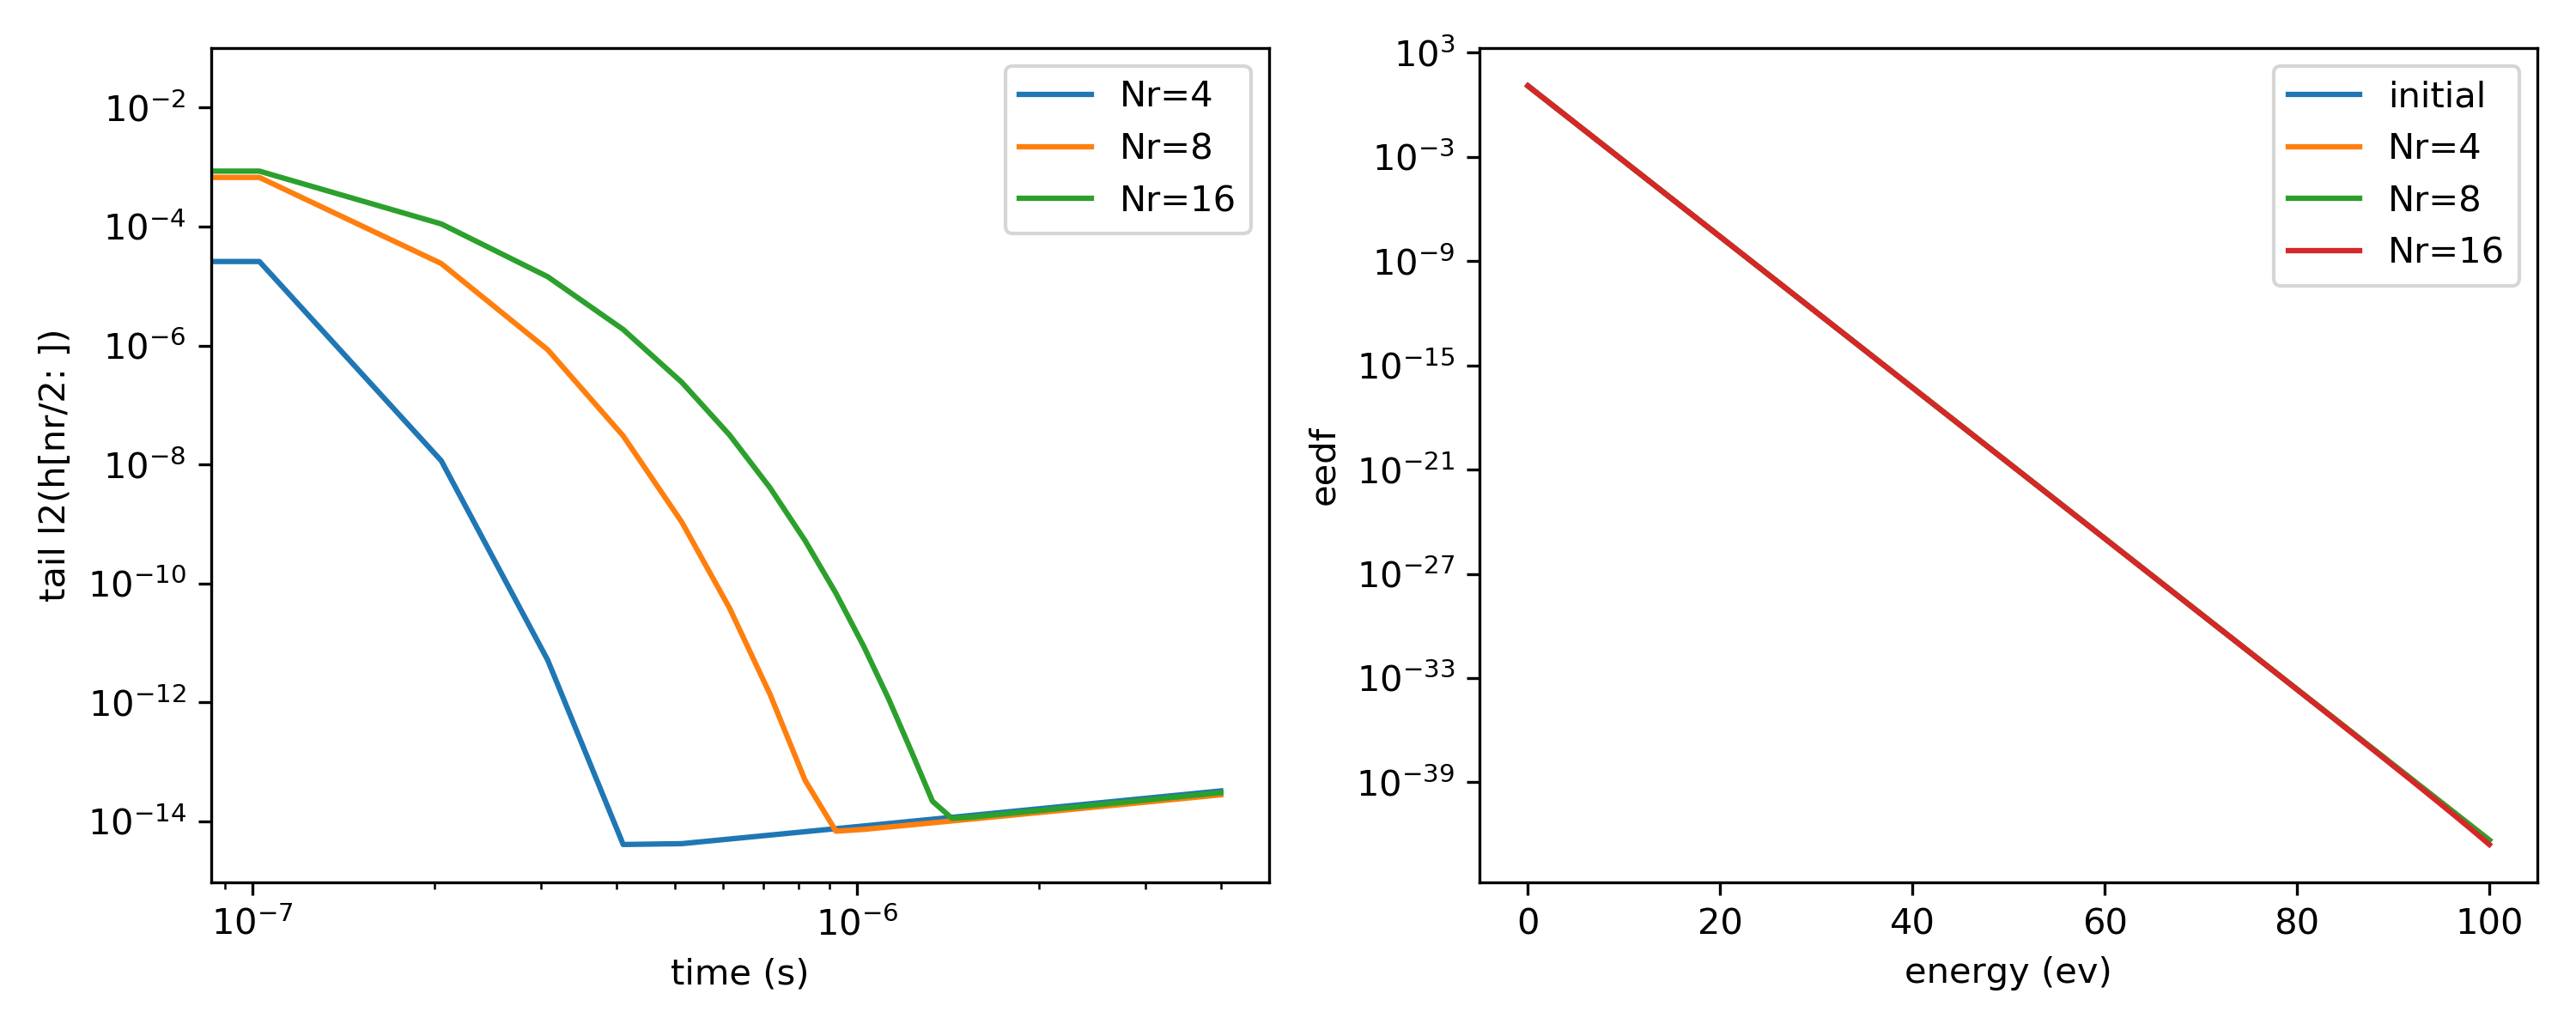
\includegraphics[width=0.48\textwidth]{figures/m_no_e_loss_aiso_test_1ev_4e-6_l2.png}
	\end{figure}
\end{frame}


%\begin{frame}
%\frametitle{V-space solver (with operator splitting)}
%\begin{columns}
%	\begin{column}{0.5\textwidth}
%		\begin{center}
%			\tiny
%			\begin{align*}
%			\partial_t f + \vect{E}\cdot \nabla_{\vect{v}} f = C[f]
%			\end{align*}
%			\begin{align*}
%			&\left\{
%			\begin{aligned}
%			\partial_t f^{(0)} + \vect{E}\cdot \nabla_{\vect{v}} f^{(0)} &= 0, \quad t_n < t \leq t_n + \frac12 \Delta t \\
%			f^{(0)}\of{t_n} &= f\of{t_n}
%			\end{aligned}
%			\right.
%			\\
%			&\left\{
%			\begin{aligned}
%			\partial_t f^{(1)} &= C[f^{(1)}], \quad t_n < t \leq t_n + \Delta t \\
%			f^{(1)}\of{t_n} &= f^{(0)}\of{t_n + \frac12 \Delta t}
%			\end{aligned}
%			\right.
%			\\
%			&\left\{
%			\begin{aligned}
%			\partial_t f^{(2)} + \vect{E}\cdot \nabla_{\vect{v}} f^{(2)} &= 0, \quad t_n + \frac12 \Delta t < t \leq t_n + \Delta t  \\
%			f^{(2)}\of{t_n} &= f^{(1)}\of{t_n + \Delta t}
%			\end{aligned}
%			\right.
%			\\
%			& f\of{t_n + \Delta t} = f^{(2)}\of{t_n + \Delta t}
%			\end{align*}
%		\end{center}
%	\end{column}
%	\begin{column}{0.5\textwidth}  %%<--- here
%		\begin{center}
%			Overall algorithm: given $\vect{v}_0$, $a_{klm}$ at $t_n$:
%			\begin{enumerate}
%				\item $\vect{v}_0 \leftarrow \vect{v}_0 - \frac{q_e}{m_e}\myint_{t_n}^{t_n+\frac12 \Delta t} \vect{E}\of{\tau} d\tau$
%				\item Solve collision op.  from $t_0$ to $t_0 + \Delta t$
%				\item compute $\tilde{v}_0$ from updated $f$
%				\item Project $f$ from $v_0$ to  $\tilde{v}_0$ update $v_0\leftarrow \tilde{v}_0$
%				\item If temperature increased project to higher $v_{th}$.
%				\item $\vect{v}_0 \leftarrow \vect{v}_0 - \frac{q_e}{m_e}\myint_{t_n+\frac12 \Delta t}^{t_n + \Delta t} \vect{E}\of{\tau} d\tau$
%			\end{enumerate}
%		\end{center}
%	\end{column}
%\end{columns}
%\end{frame}

\begin{frame}
	\frametitle{Eulerian approach with linear splines}
	E=10V/m along z-axis, with elastic + ionization reactions, T=$10^{-4}$ s
	\begin{figure}
		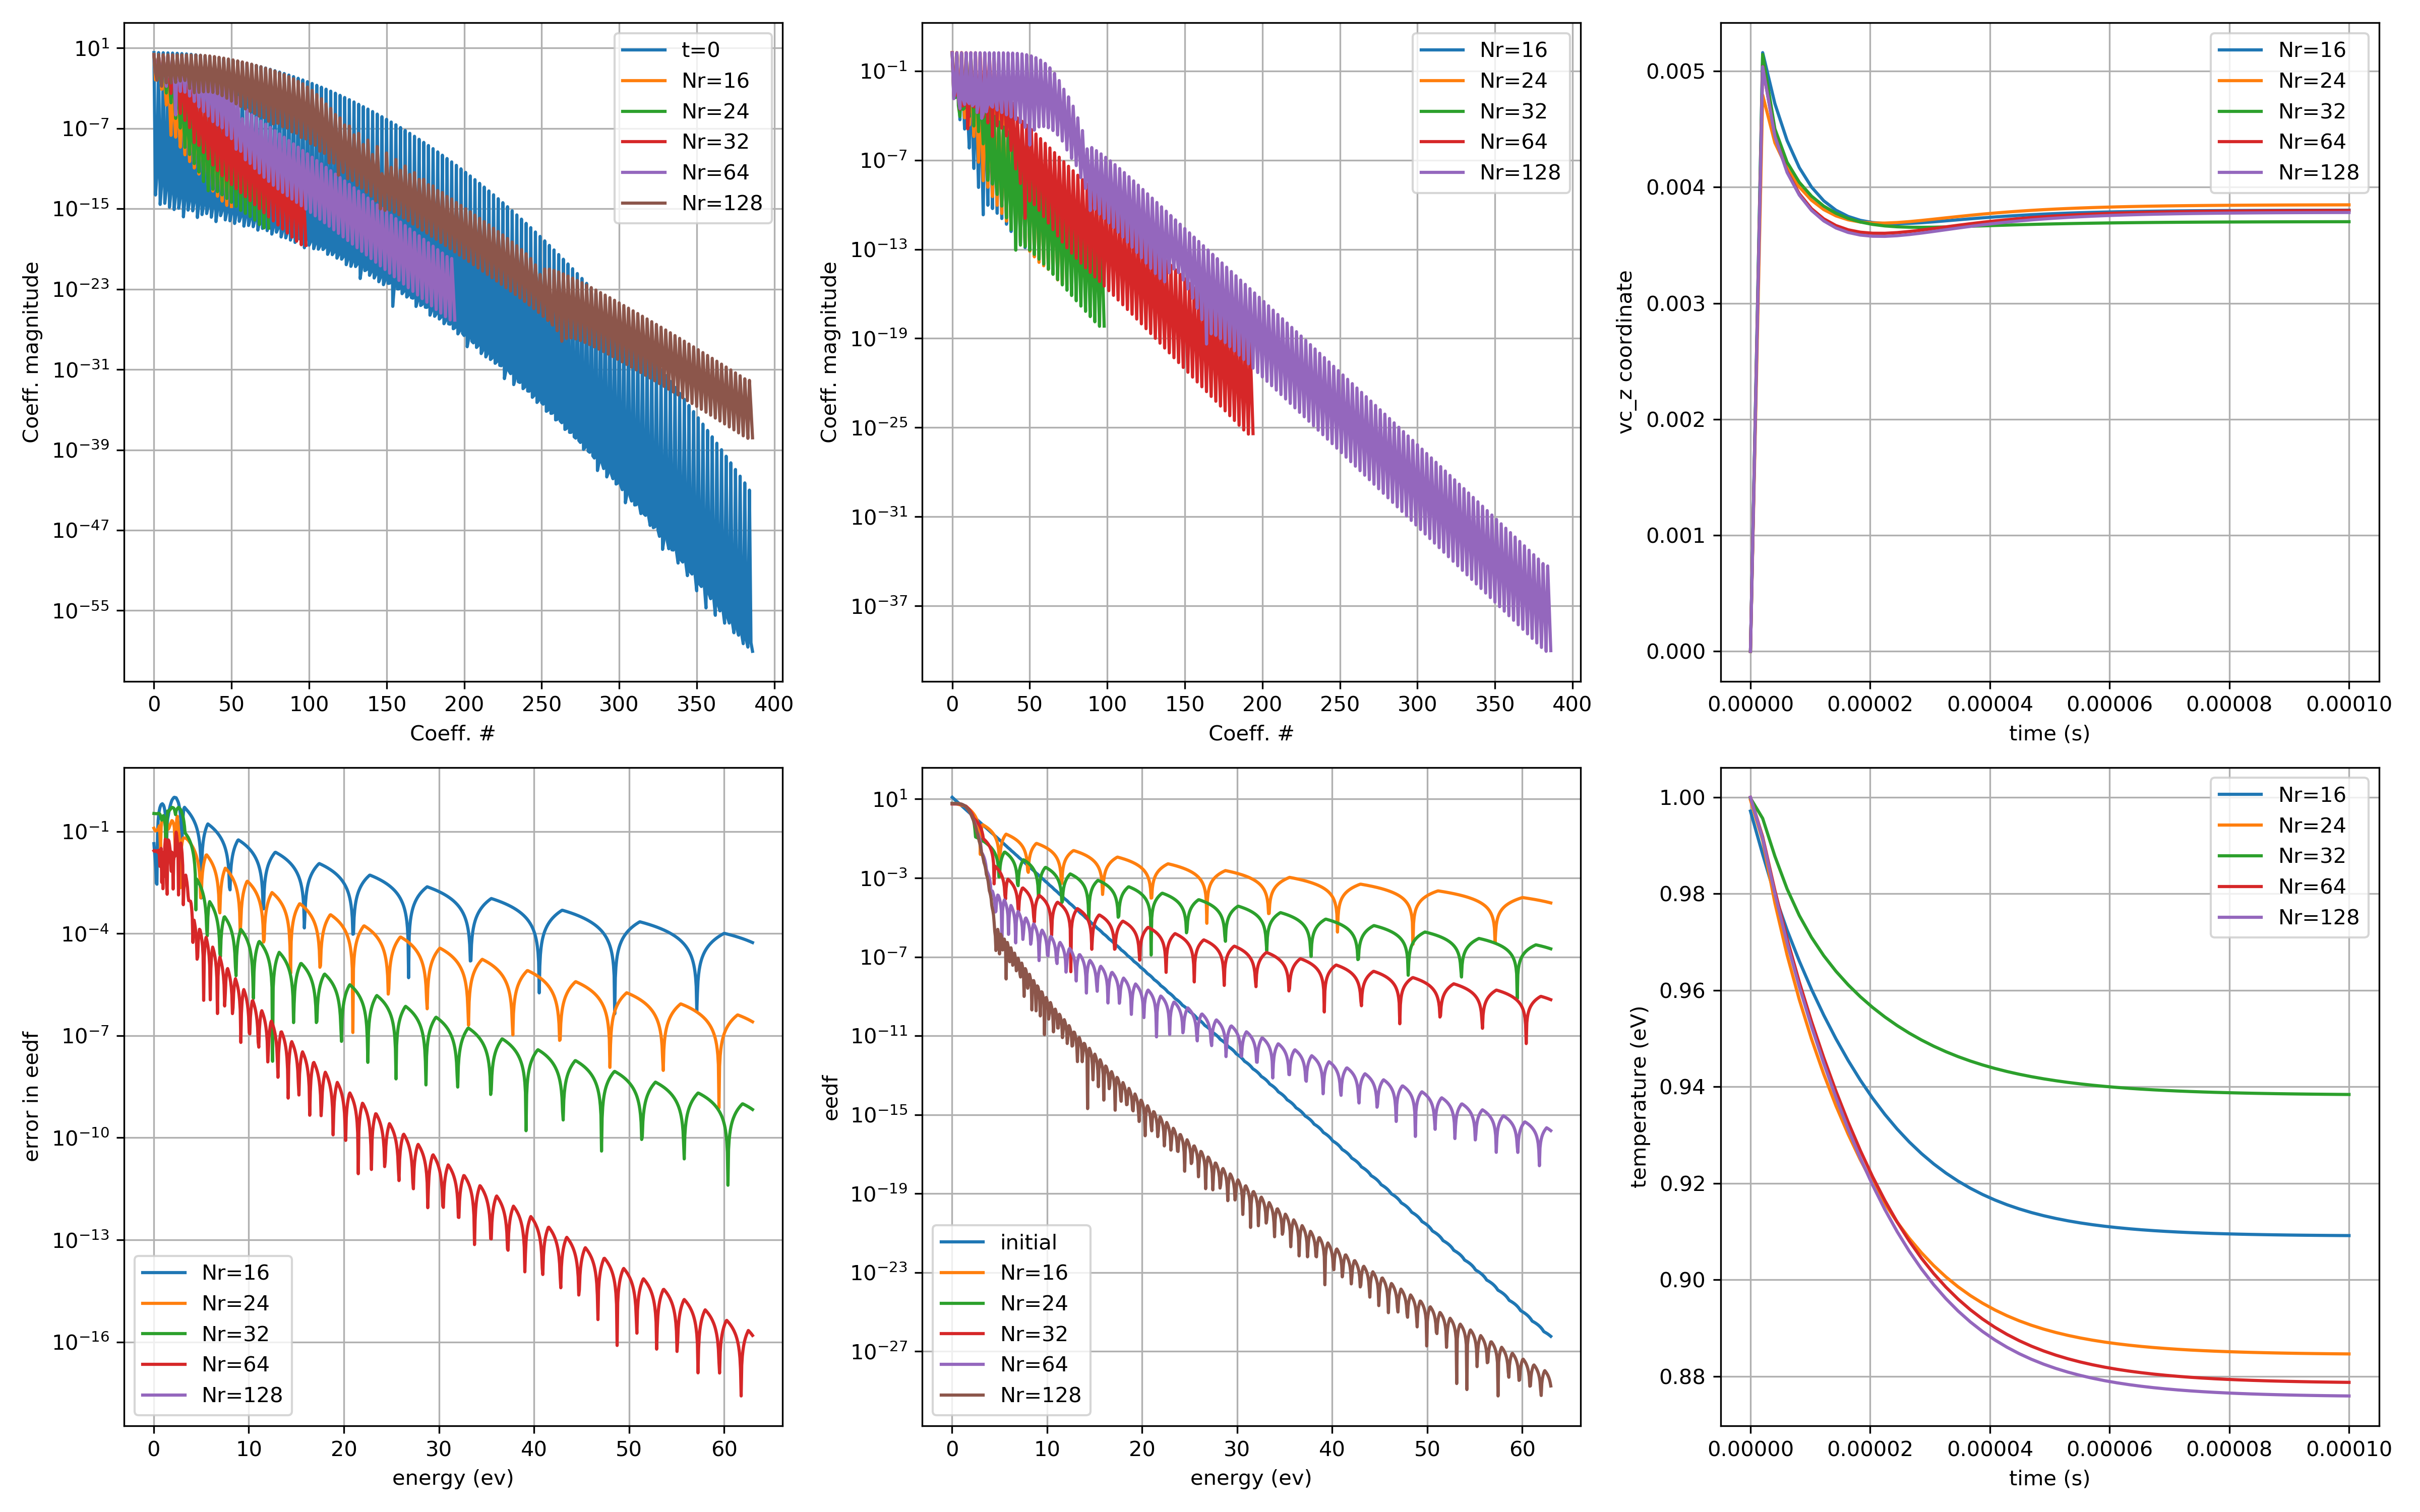
\includegraphics[width=0.65\textwidth]{figures/b_1ev_10Vpm_vspace_coeff.png}
	\end{figure}
\end{frame}

%\begin{frame}
%	\frametitle{Maxwell : Elastic + Ionization + advection}
%	\begin{figure}
%		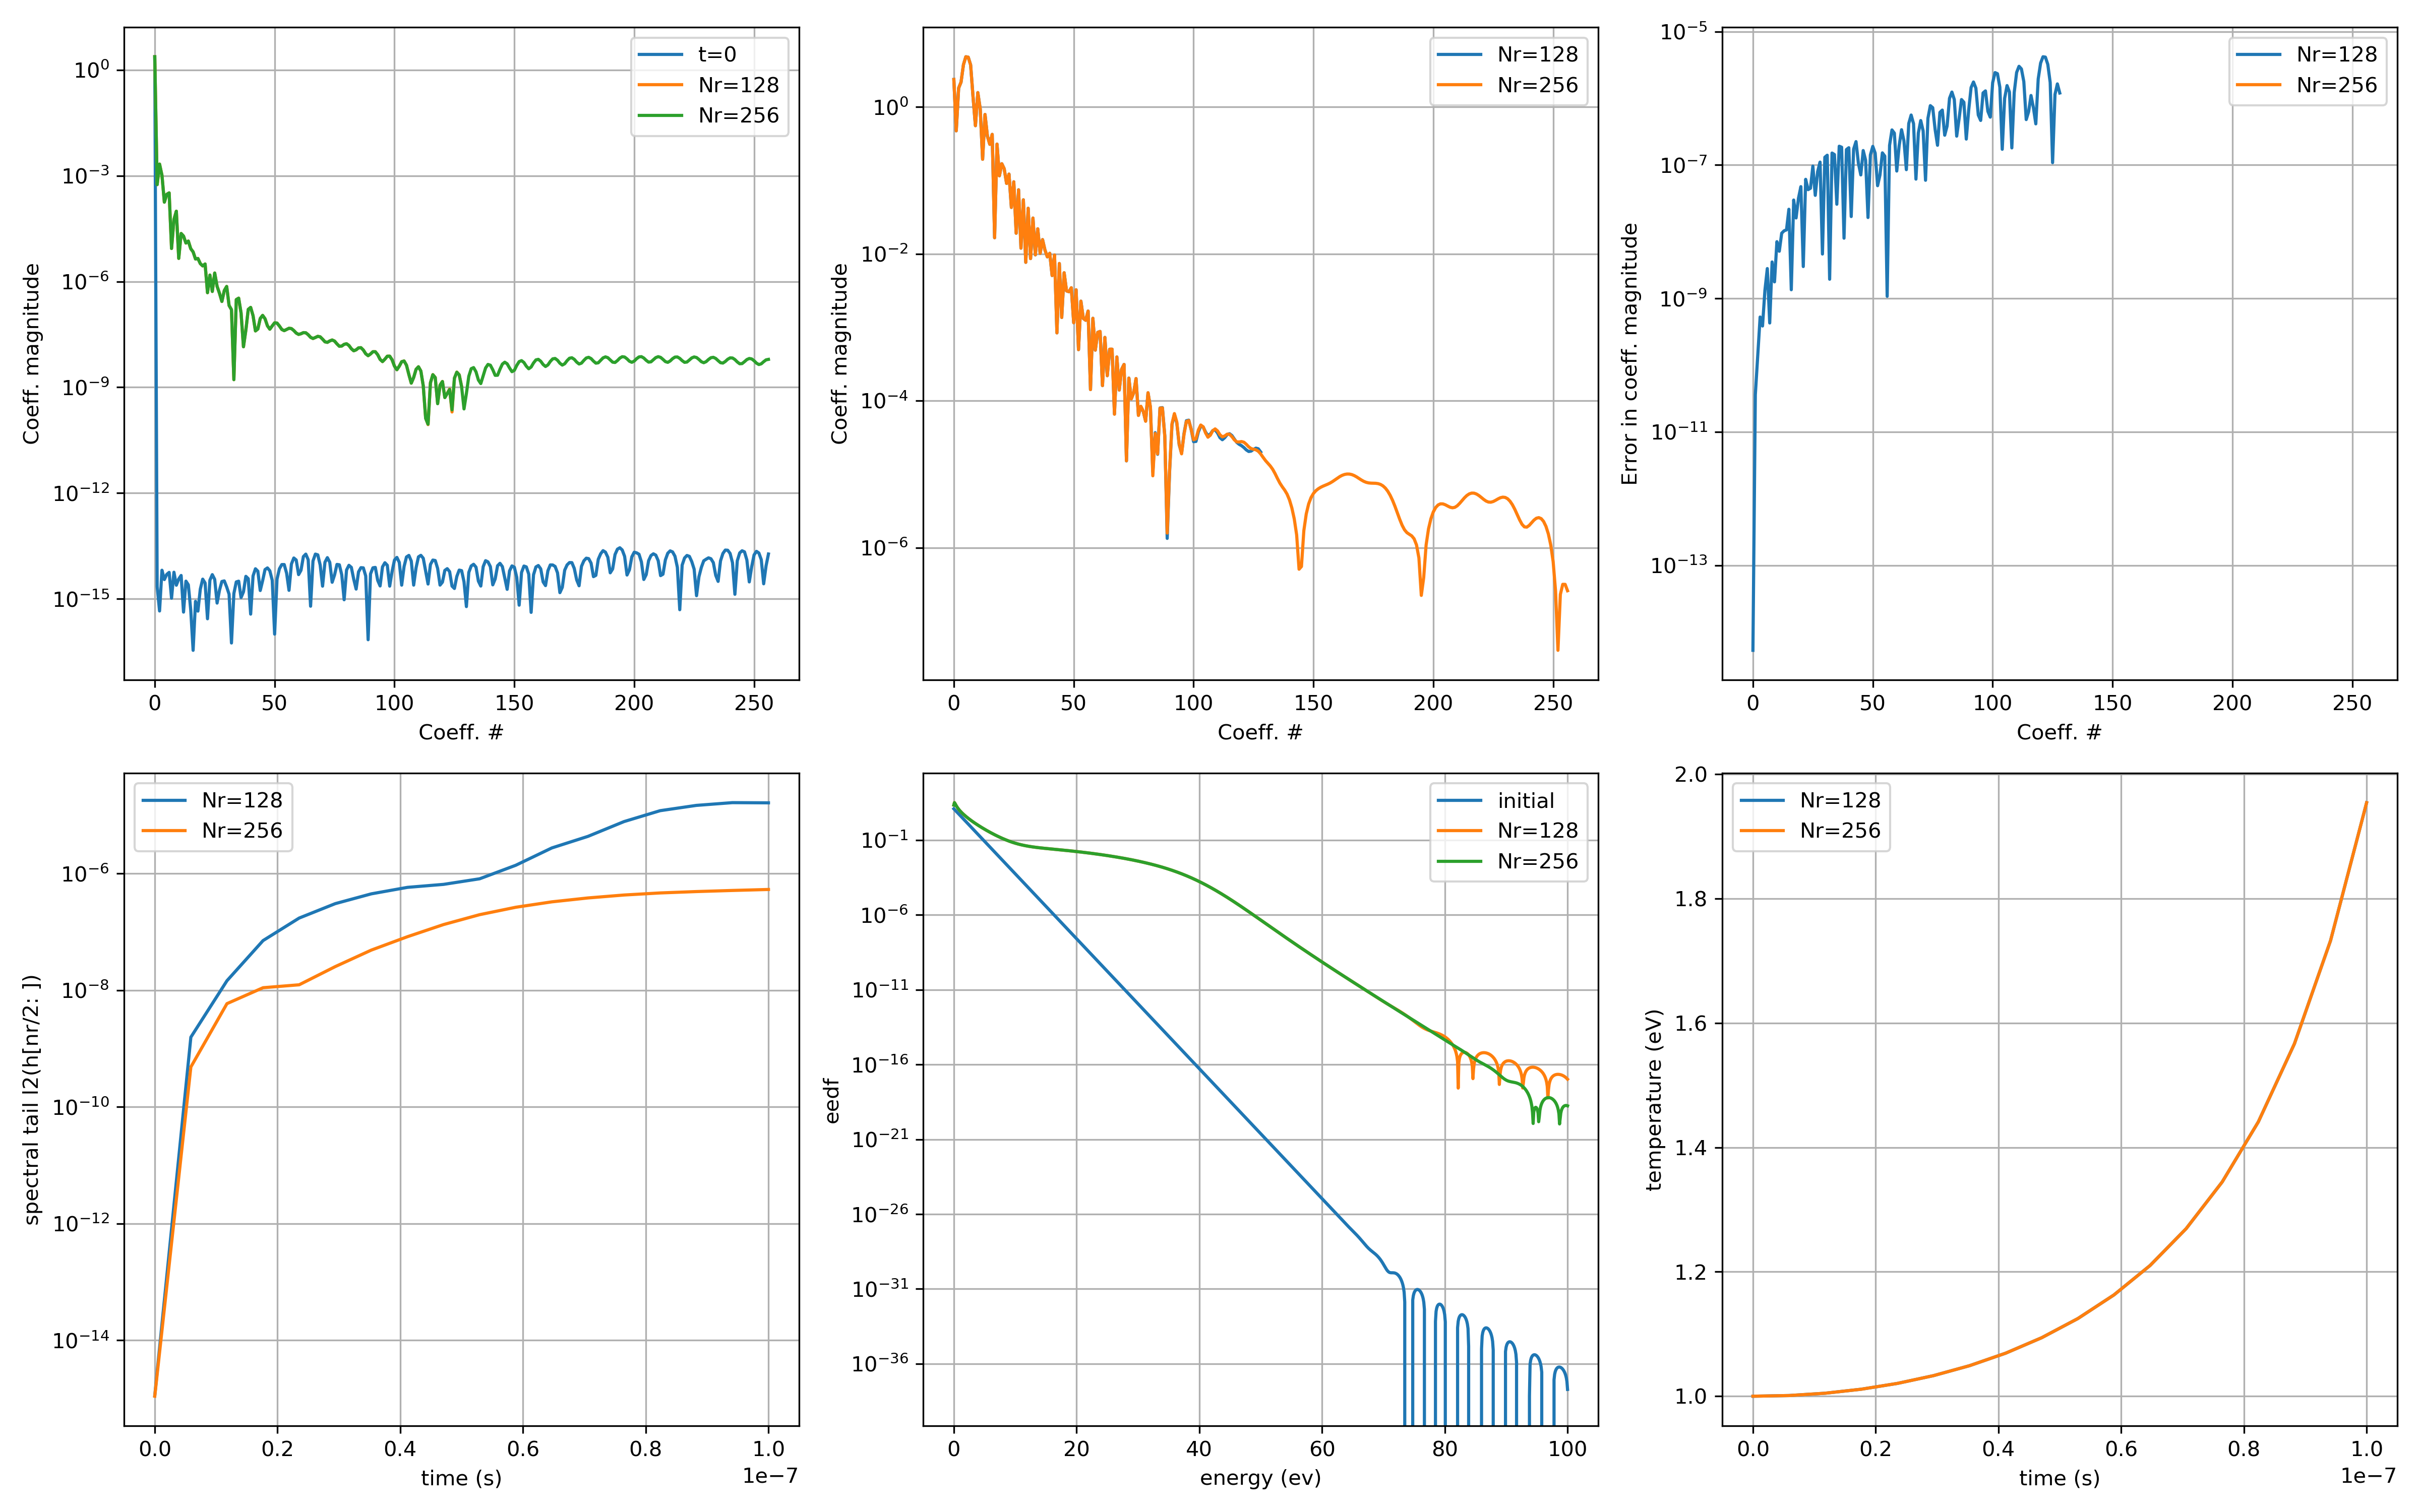
\includegraphics[width=0.7\textwidth]{figures/m_test_vspace_coeff.png}
%	\end{figure}
%\end{frame}



\begin{frame}
%\frametitle{Steady-State solutions for orthogonal polynomials}
\begin{itemize}
\item Discretized system of equations 
\begin{align*}
\frac{d \vect{h}}{dt} + E \vect{h} = C \vect{h}
\end{align*}
admits a steady state solution:
\begin{align*}
\frac{\vect{h}_\ast}{h_0} = 
\left( \left(C_{00} + \vect{c}_{\ast 0}^T \frac{\vect{h}_\ast}{h_0} \right) I
- \left( C_{\ast\ast} - E_{\ast\ast} \right) \right)^{-1}
\left( \vect{c}_{0\ast} - \vect{e}_{0\ast} \right)
\end{align*}
where
\begin{align*}
\vect{h} = 
\begin{pmatrix}
h_0 \\ \vect{h}_\ast
\end{pmatrix}
,\quad
E = 
\begin{pmatrix}
0 & \vect{0}^T \\
\vect{e}_{0\ast} & E_{\ast\ast}
\end{pmatrix}
,\quad
C = 
\begin{pmatrix}
C_{00} & \vect{c}_{\ast 0}^T \\
\vect{c}_{0\ast} & C_{\ast\ast}
\end{pmatrix}
\end{align*}

\item Solving using fixed-point iteration (typically converges in $<5$ iterations)
\begin{align*}
\bar{\vect{h}}^{n+1} = 
\left( \left(C_{00} + \vect{c}_{\ast 0}^T \bar{\vect{h}}^{n} \right) I
- \left( C_{\ast\ast} - E_{\ast\ast} \right) \right)^{-1}
\left( \vect{c}_{0\ast} - \vect{e}_{0\ast} \right)
\end{align*}
\end{itemize}
%	\begin{figure}
%		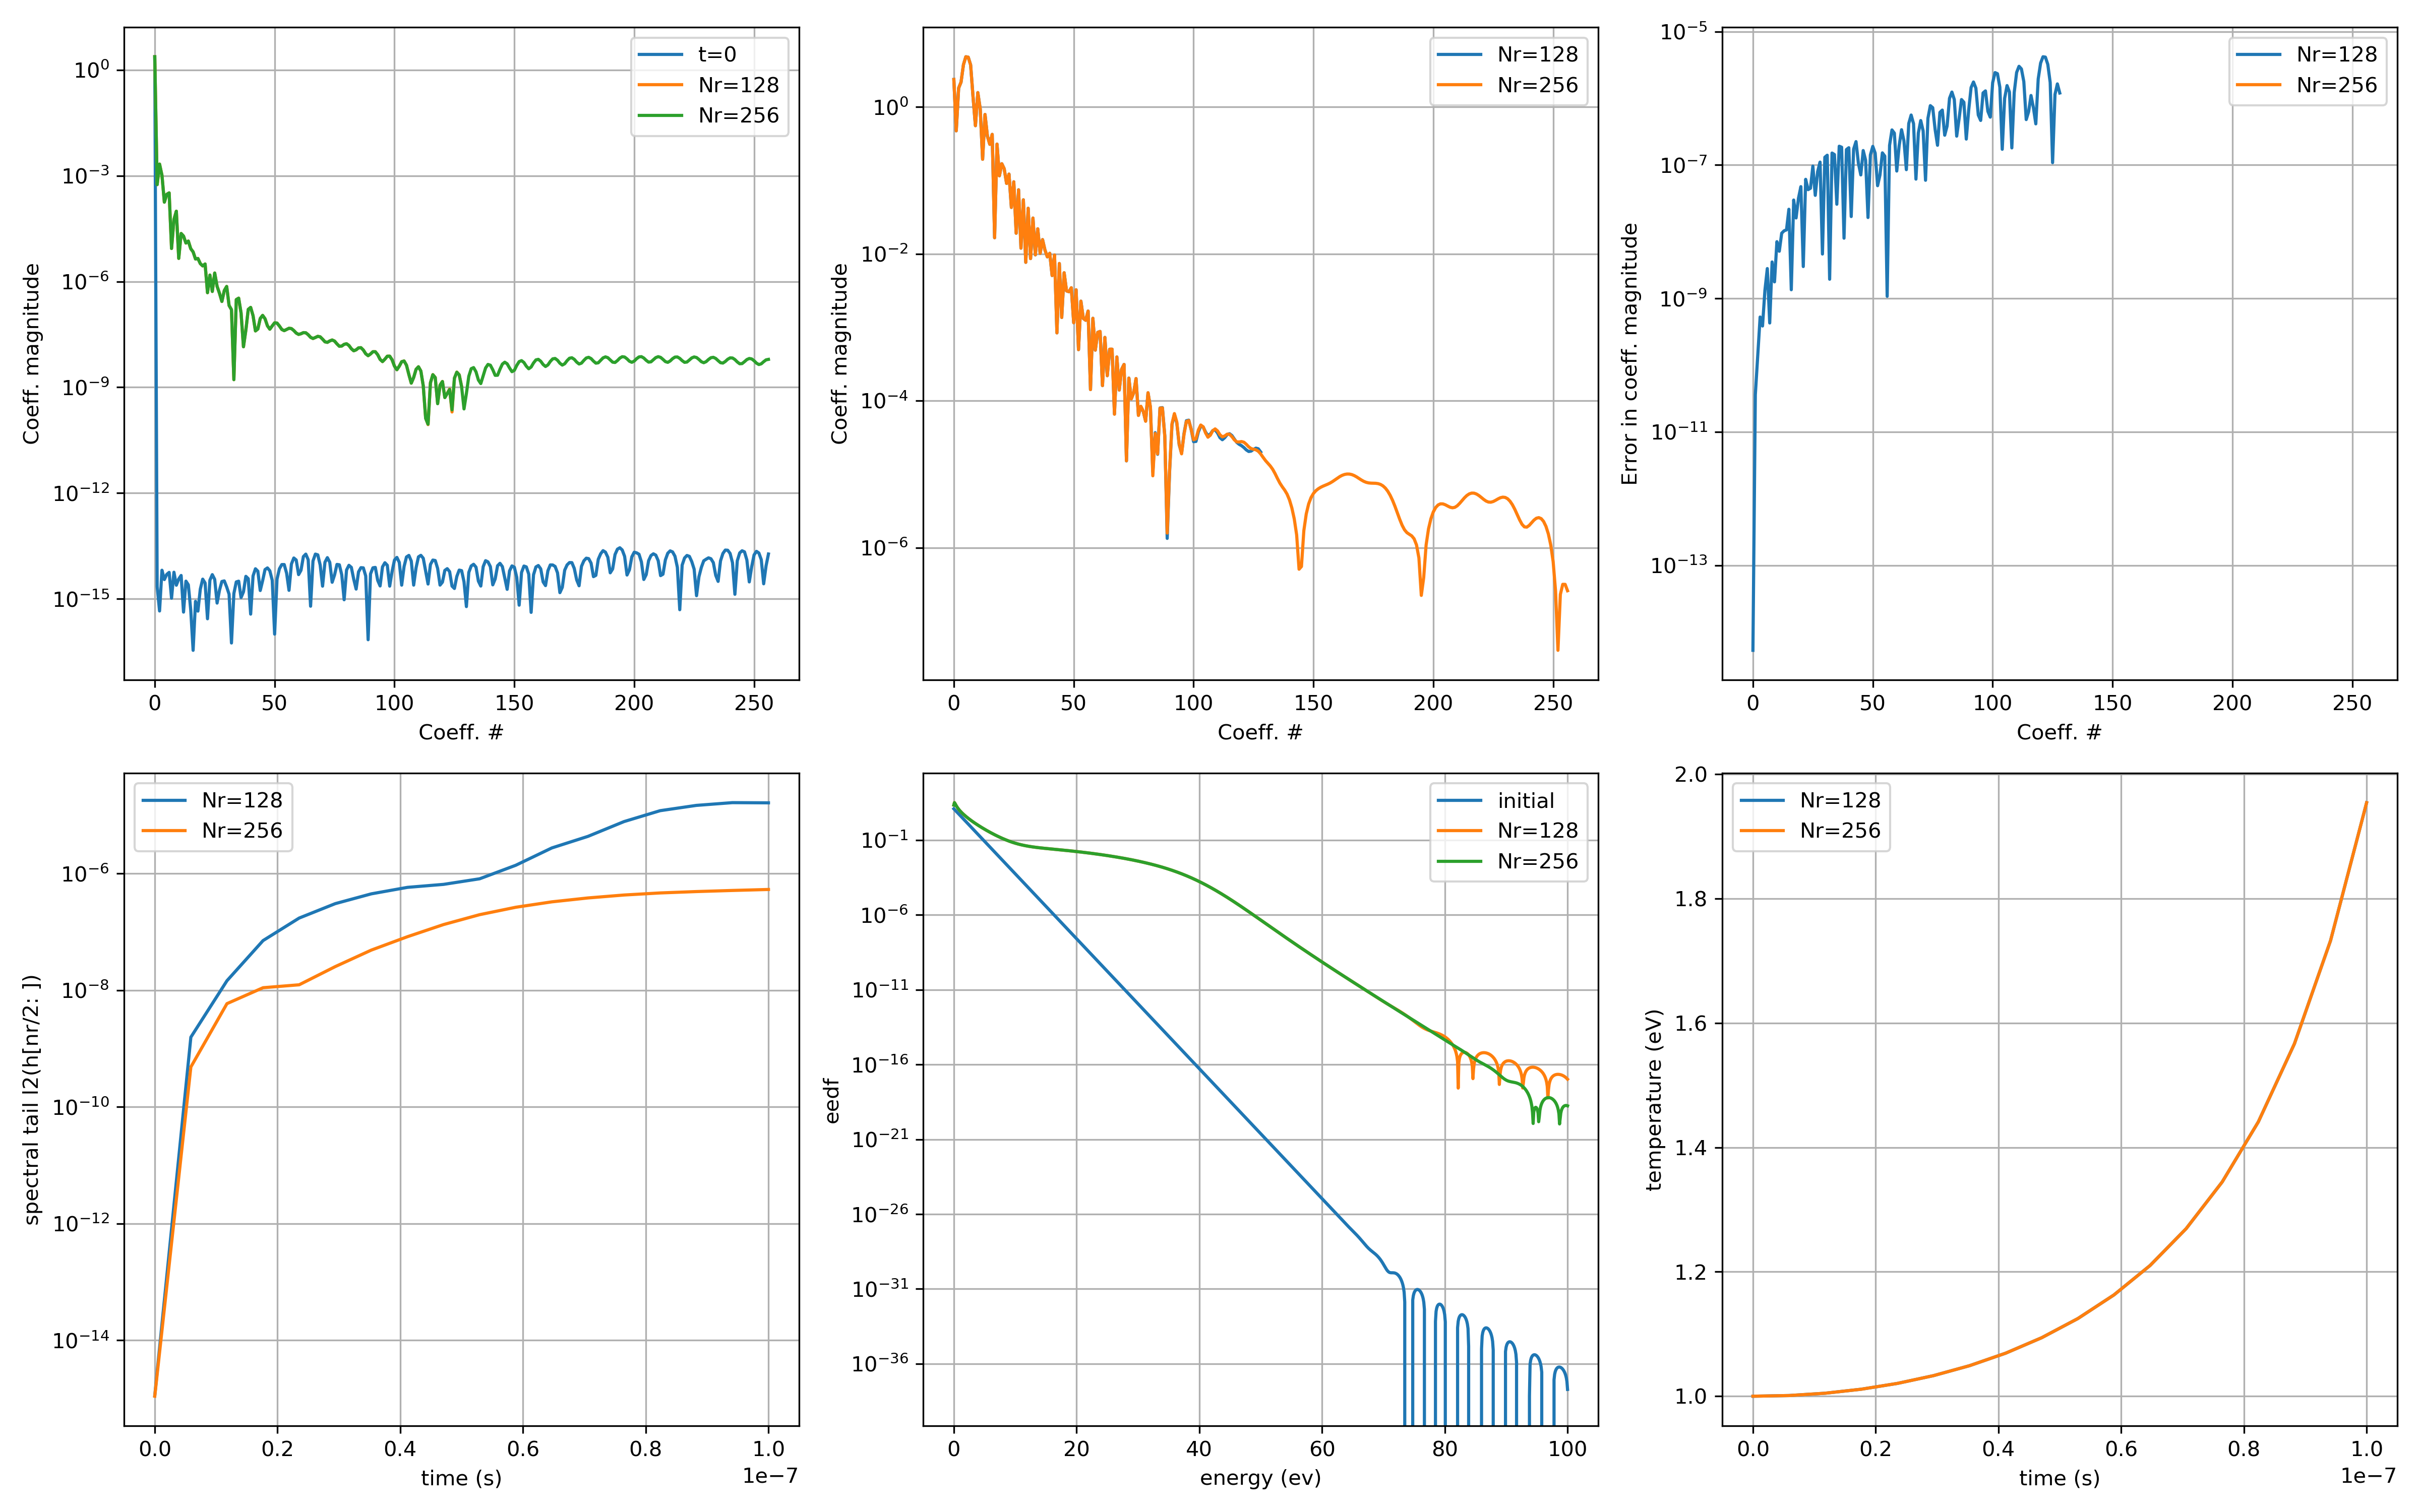
\includegraphics[width=0.7\textwidth]{figures/m_test_vspace_coeff.png}
%\end{figure}
\end{frame}



\begin{frame}
Validation against Bolsig+ results:
\begin{enumerate}
\item Only elastic collisions with constant cross sections ($E=10$ V/m)
\begin{enumerate}
\item Convergence with increasing $N_r$ (number of radial polynomials)
\item Sensitivity to basis thermal velocity (for $Nr = 64$)
\item Sensitivity to choice of polynomials: Maxwell vs Laguerre (for $Nr = 64$)
\end{enumerate}
\item Only elastic collisions with experiment-fitted cross sections
\begin{enumerate}
\item Sweep through $E = 1, 10, 100, 500, 1000$ V/m
\end{enumerate}
\item Elastic and ionization collisions with experiment-fitted cross sections
\begin{enumerate}
\item Sweep through $E = 1, 10, 100, 500, 1000, 5000, 10000$ V/m
\end{enumerate}
\end{enumerate}


Some notes:
\begin{itemize}
\item We use 8 quadrature points for integration over all angular dimensions, and 200 quadrature points for radial direction
\item For basis thermal velocity values from Bolsig+ results are used unless otherwise stated
\item Swarm parameters are computed quite roughly using sampled distributions and trapezoidal integration
\end{itemize}
\end{frame}



\begin{frame}

\begin{figure}
1. Only elastic collisions with constant cross sections ($E=10$ V/m):
\\ 
1.1 Convergence with increasing $N_r$ (number of radial polynomials)

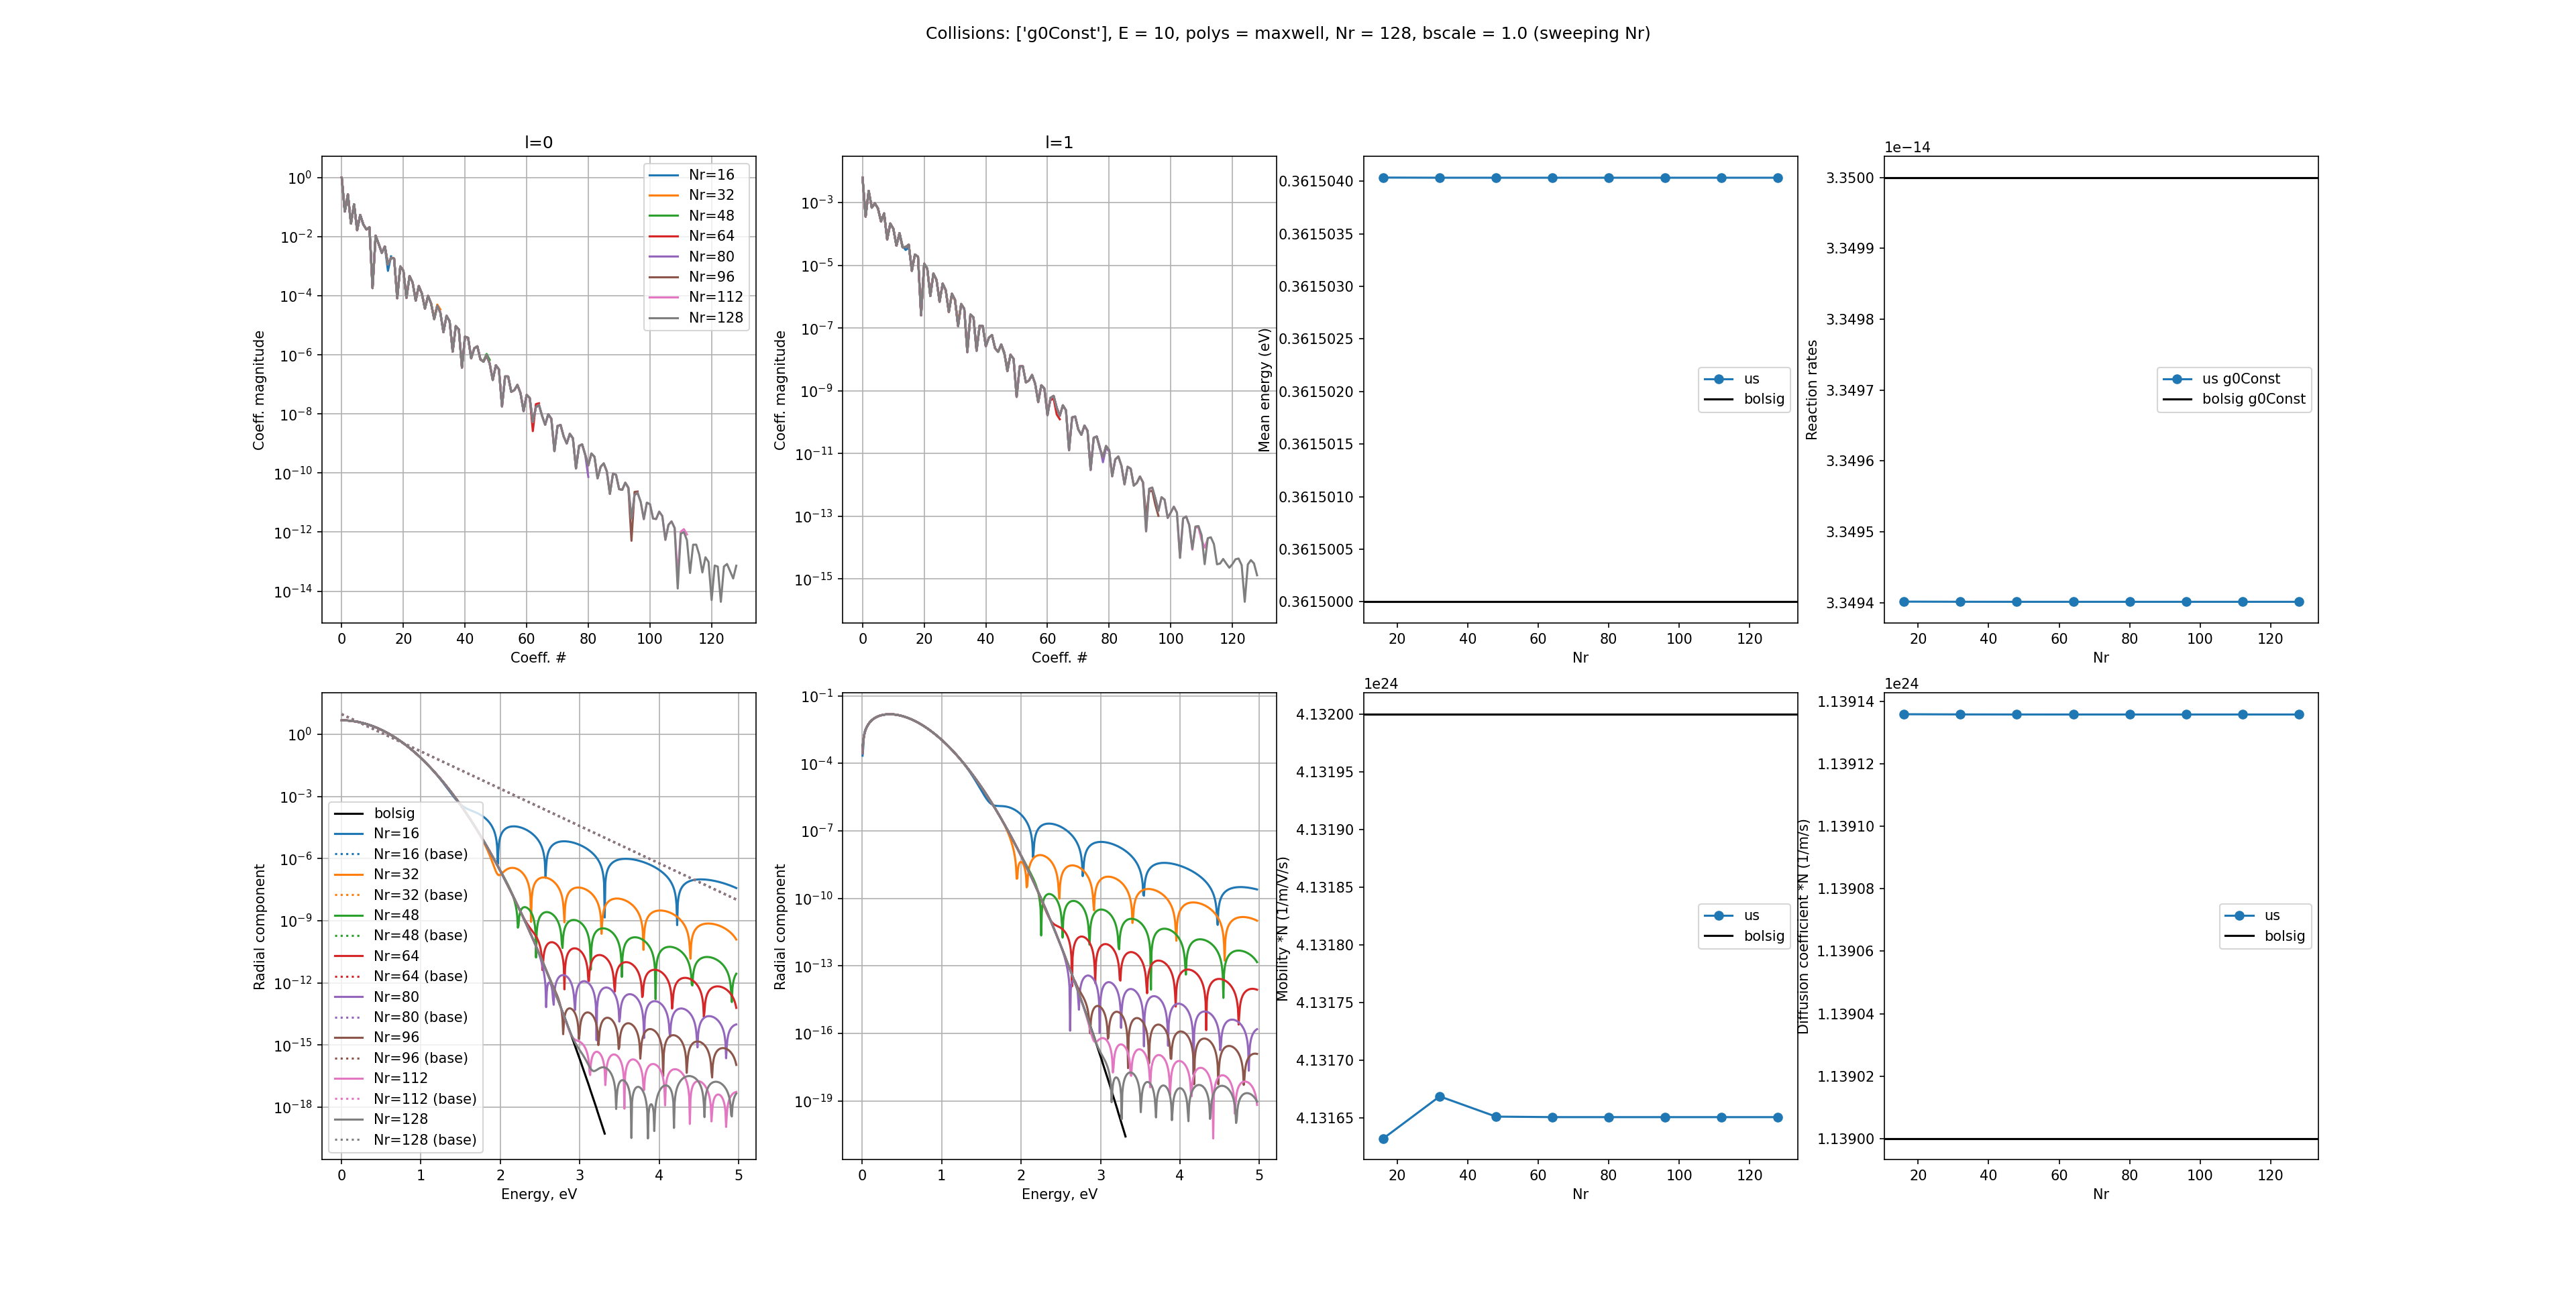
\includegraphics[width=\textwidth]{maxwell_vs_bolsig_g0Const_E10_poly_maxwell_nrsweep_bscale1.png}
\end{figure}

\end{frame}



\begin{frame}

\begin{figure}
1. Only elastic collisions with constant cross sections ($E=10$ V/m):
\\ 
1.2 Sensitivity to basis thermal velocity (for $Nr = 64$)

\includegraphics[width=\textwidth]{maxwell_vs_bolsig_g0Const_E10_poly_maxwell_nr64_bscalesweep.png}
\end{figure}

\end{frame}



\begin{frame}

\begin{figure}
1. Only elastic collisions with constant cross sections ($E=10$ V/m):
\\ 
1.3 Sensitivity to choice of polynomials: Maxwell vs Laguerre (for $Nr = 64$)

\includegraphics[width=\textwidth]{{maxwell_vs_bolsig_g0Const_E10_poly_laguerre_nr64_bscale1.0_sweeping_radial_poly}.png}
\end{figure}

\end{frame}



\begin{frame}

\begin{figure}
2. Only elastic collisions with experiment-fitted cross sections
\\ 
2.1 $E=1$ V/m

\includegraphics[width=\textwidth]{maxwell_vs_bolsig_g0_E1_poly_maxwell_nrsweep_bscale1.png}
\end{figure}

\end{frame}



\begin{frame}

\begin{figure}
2. Only elastic collisions with experiment-fitted cross sections
\\ 
2.2 $E=10$ V/m

\includegraphics[width=\textwidth]{{maxwell_vs_bolsig_g0_E10.0_poly_maxwell_nr128_bscale1.0_sweeping_Nr}.png}
\end{figure}

\end{frame}



\begin{frame}

\begin{figure}
2. Only elastic collisions with experiment-fitted cross sections
\\ 
2.3 $E=100$ V/m

\includegraphics[width=\textwidth]{{maxwell_vs_bolsig_g0_E100.0_poly_maxwell_nr128_bscale1.0_sweeping_Nr}.png}
\end{figure}

\end{frame}



\begin{frame}

\begin{figure}
2. Only elastic collisions with experiment-fitted cross sections
\\ 
2.4 $E=500$ V/m

\includegraphics[width=\textwidth]{{maxwell_vs_bolsig_g0_E500.0_poly_maxwell_nr128_bscale1.0_sweeping_Nr}.png}
\end{figure}

\end{frame}



\begin{frame}

\begin{figure}
2. Only elastic collisions with experiment-fitted cross sections
\\ 
2.5 $E=1000$ V/m (struggles to find solution)

\includegraphics[width=\textwidth]{{maxwell_vs_bolsig_g0_E1000.0_poly_maxwell_nr128_bscale1.0_sweeping_Nr}.png}
\end{figure}

\end{frame}



\begin{frame}

\begin{figure}
3. Elastic and ionization collisions with experiment-fitted cross sections
\\ 
3.1 $E=1$ V/m (for rates we display relative error now)

\includegraphics[width=\textwidth]{{maxwell_vs_bolsig_g0_g2_E1.0_poly_maxwell_nr128_bscale1.0_sweeping_Nr}.png}
\end{figure}

\end{frame}



\begin{frame}

\begin{figure}
3. Elastic and ionization collisions with experiment-fitted cross sections
\\ 
3.2 $E=10$ V/m (for rates we display relative error now)

\includegraphics[width=\textwidth]{{maxwell_vs_bolsig_g0_g2_E10.0_poly_maxwell_nr128_bscale1.0_sweeping_Nr}.png}
\end{figure}

\end{frame}



\begin{frame}

\begin{figure}
3. Elastic and ionization collisions with experiment-fitted cross sections
\\ 
3.3 $E=100$ V/m (for rates we display relative error now)

\includegraphics[width=\textwidth]{{maxwell_vs_bolsig_g0_g2_E100.0_poly_maxwell_nr128_bscale1.0_sweeping_Nr}.png}
\end{figure}

\end{frame}



\begin{frame}

\begin{figure}
3. Elastic and ionization collisions with experiment-fitted cross sections
\\ 
3.4 $E=500$ V/m (for rates we display relative error now)

\includegraphics[width=\textwidth]{{maxwell_vs_bolsig_g0_g2_E500.0_poly_maxwell_nr128_bscale1.0_sweeping_Nr}.png}
\end{figure}

\end{frame}




\begin{frame}

\begin{figure}
3. Elastic and ionization collisions with experiment-fitted cross sections
\\ 
3.5 $E=1000$ V/m (for rates we display relative error now)

\includegraphics[width=\textwidth]{{maxwell_vs_bolsig_g0_g2_E1000.0_poly_maxwell_nr128_bscale1.0_sweeping_Nr}.png}
\end{figure}

\end{frame}



\begin{frame}

\begin{figure}
3. Elastic and ionization collisions with experiment-fitted cross sections
\\ 
3.6 $E=5000$ V/m (for rates we display relative error now)

\includegraphics[width=\textwidth]{{maxwell_vs_bolsig_g0_g2_E5000.0_poly_maxwell_nr128_bscale1.0_sweeping_Nr}.png}
\end{figure}

\end{frame}



\begin{frame}

\begin{figure}
3. Elastic and ionization collisions with experiment-fitted cross sections
\\ 
3.7 $E=10000$ V/m (for rates we display relative error now)

\includegraphics[width=\textwidth]{{maxwell_vs_bolsig_g0_g2_E10000.0_poly_maxwell_nr128_bscale1.0_sweeping_Nr}.png}
\end{figure}

\end{frame}



\begin{frame}
Some conlcusions and observations:
\begin{enumerate}
\item Only elastic collisions with constant cross sections ($E=10$ V/m)
\begin{enumerate}
\item Convergence with increasing $N_r$ (number of radial polynomials)
\\ $\rightarrow$ converges nicely
\item Sensitivity to basis thermal velocity (for $Nr = 64$)
\\ $\rightarrow$ strongly affects tail resolution but unclear how to pick
\item Sensitivity to choice of polynomials: Maxwell vs Laguerre (for $Nr = 64$)
\\ $\rightarrow$ no big difference noted, Maxwell appear slightly better
\end{enumerate}
\item Only elastic collisions with experiment-fitted cross sections
\begin{enumerate}
\item Sweep through $E = 1, 10, 100, 500, 1000$ V/m
\\ $\rightarrow$ seem to converge but slowly than in const case, unstable for high voltages (1000 V/m, not physically relevant without ionization?)
\end{enumerate}
\item Elastic and ionization collisions with experiment-fitted cross sections
\begin{enumerate}
\item Sweep through $E = 1, 10, 100, 500, 1000, 5000, 10000$ V/m
\\ $\rightarrow$ for low voltages coincide with elastic only case because no ionization is triggered
\\ $\rightarrow$ for intermediate voltages high errors in rates since tails are not well resolved
\\ $\rightarrow$ for high voltages accuracy of rates improves since ionization now affects not only tails but entire distributions
\\ $\rightarrow$ overall convergence seem to be slow (not respecting numerically discontinuous character of ionization cross section?)
\end{enumerate}
\end{enumerate}

\end{frame}


\begin{frame}[fragile]
Validation against Bolsig+ with linear B-splines.
\begin{align*}
\partial_t \hat{f} &= -\left(u^T C \hat{f}\right) \hat{f} + (C-E) \hat{f} \\
\end{align*} with enforced constraint $u^T \hat{f} -1 = 0 \ \ \forall t>0$. 
\begin{itemize}
	\item We evolve the normalized distribution function until the steady state is reached. 
	\item Used 4 quadrature points for each angular direction, radial quadrature points $2N_r$ where $N_r$ denotes the number of polynomials in the radial direction. 
	\item Linear splines with knot domain adjusted to match the energy range reported by the bolsig+ code. 
\end{itemize}
\end{frame}

\begin{frame}
	\begin{itemize}
		\item Only with elastic collisions with increasing $\vect{E}$ (curve-fitted cross sections to LXCAT).
	\end{itemize}
	\begin{center}
		\only<+>{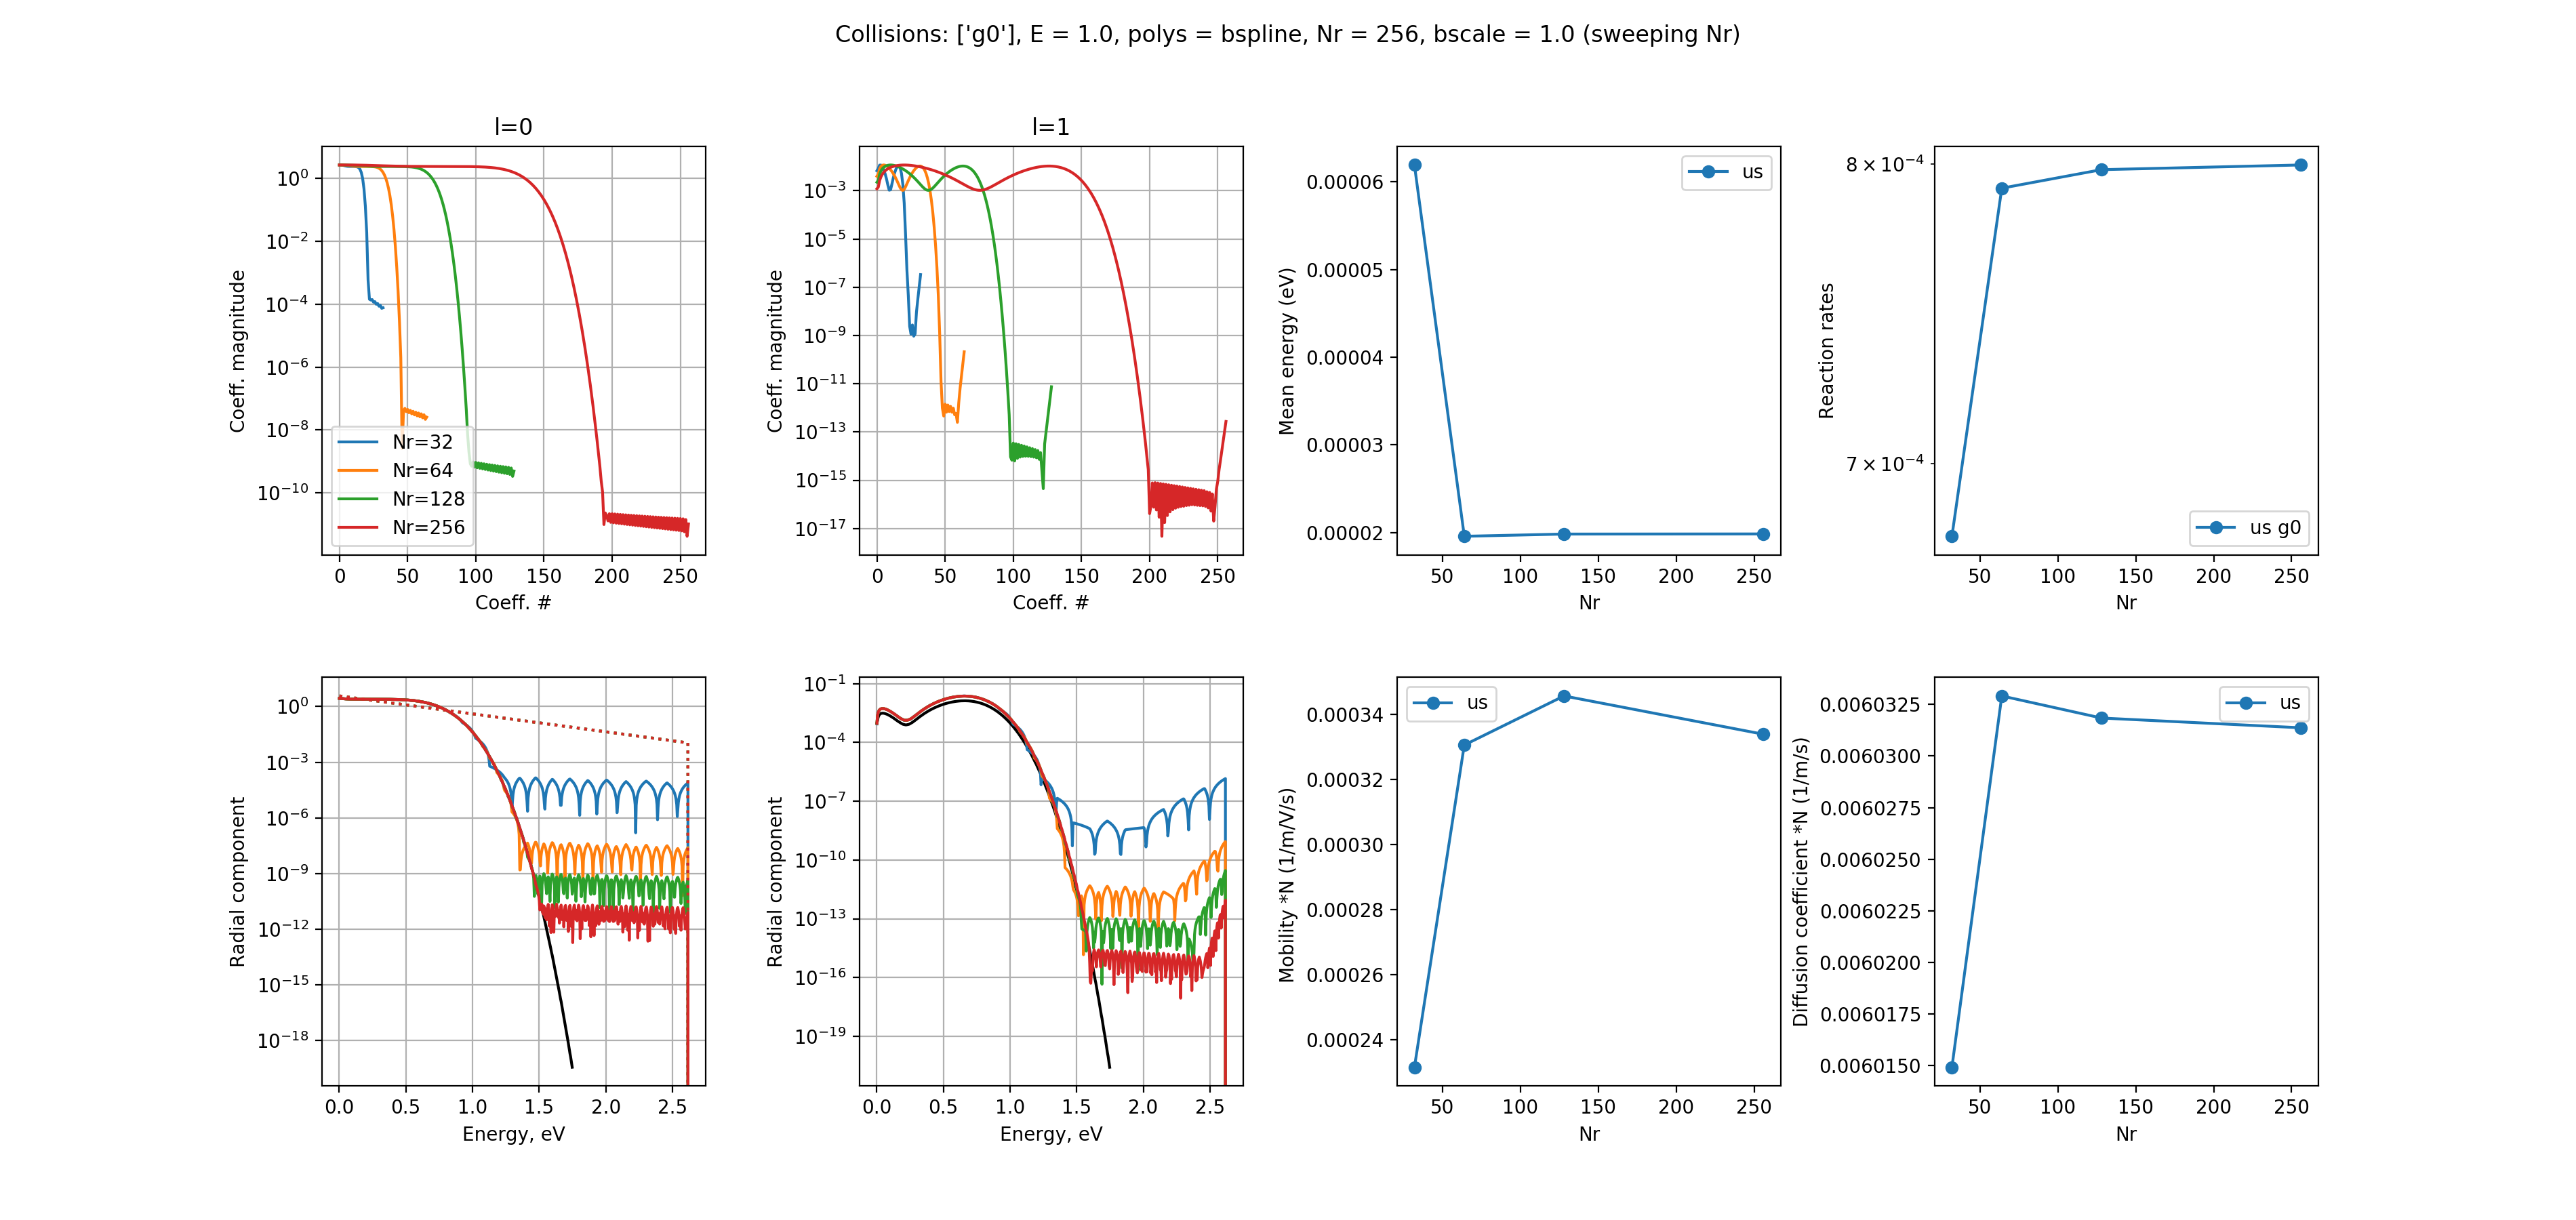
\includegraphics[width=\textwidth]{figures/maxwell_vs_bolsig_g0_E1.0_poly_bspline_nr256_bscale1.0_sweeping_Nr.png}}
		\only<+>{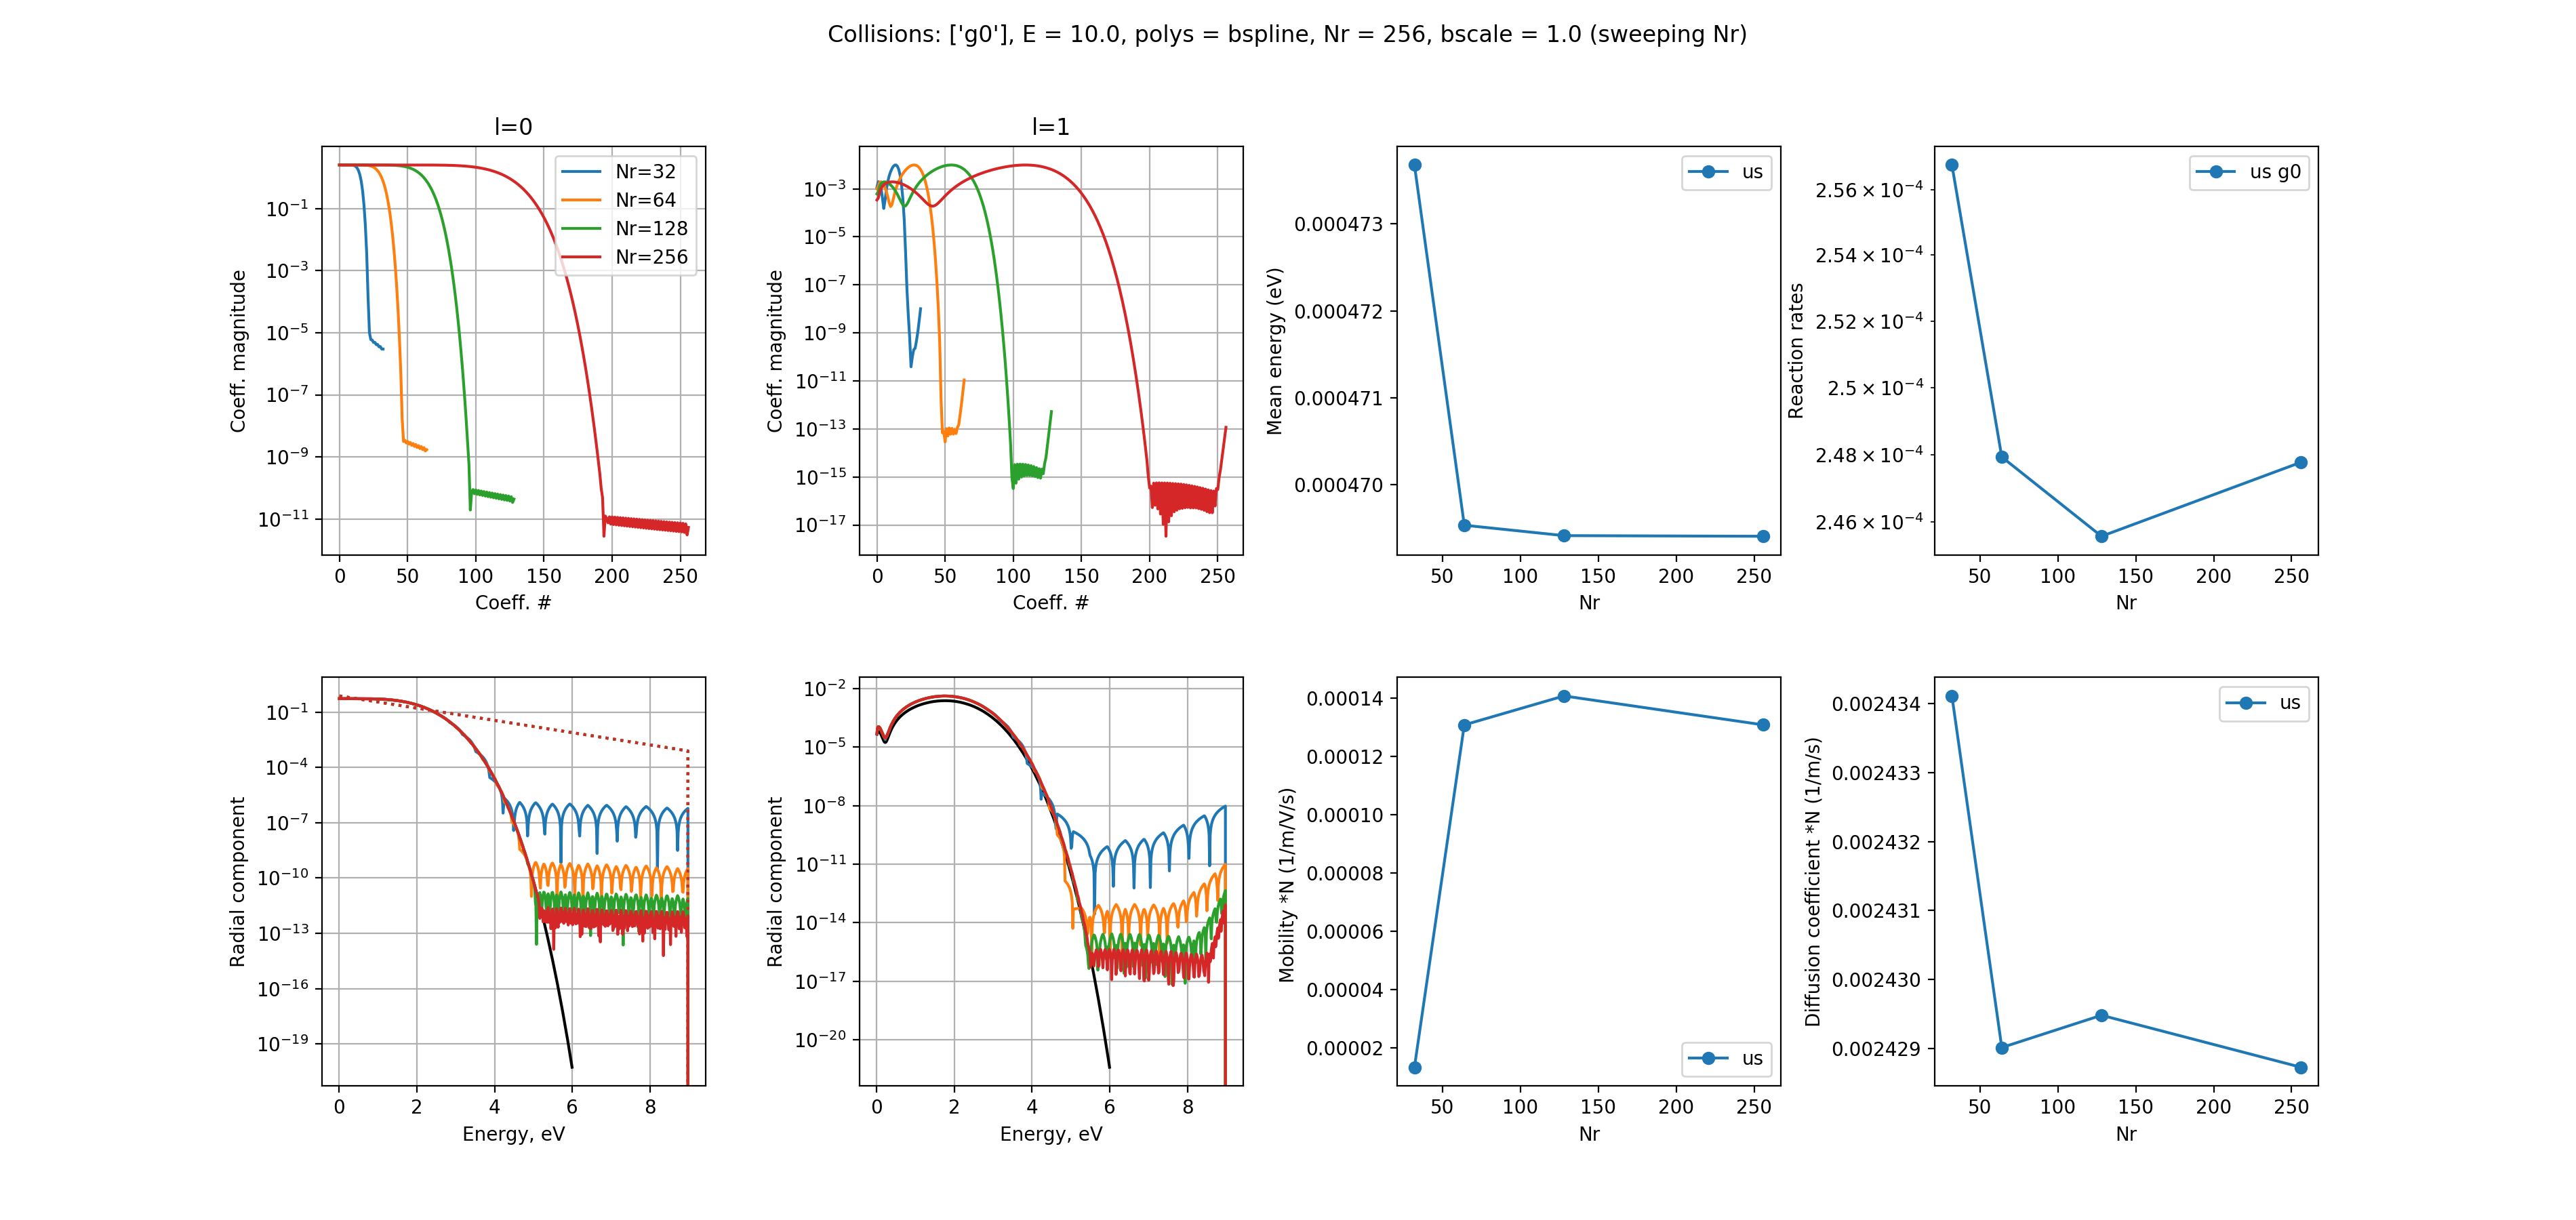
\includegraphics[width=\textwidth]{figures/maxwell_vs_bolsig_g0_E10.0_poly_bspline_nr256_bscale1.0_sweeping_Nr.png}}
		\only<+>{\includegraphics[width=\textwidth]{figures/maxwell_vs_bolsig_g0_E100.0_poly_bspline_nr256_bscale1.0_sweeping_Nr.png}}
		\only<+>{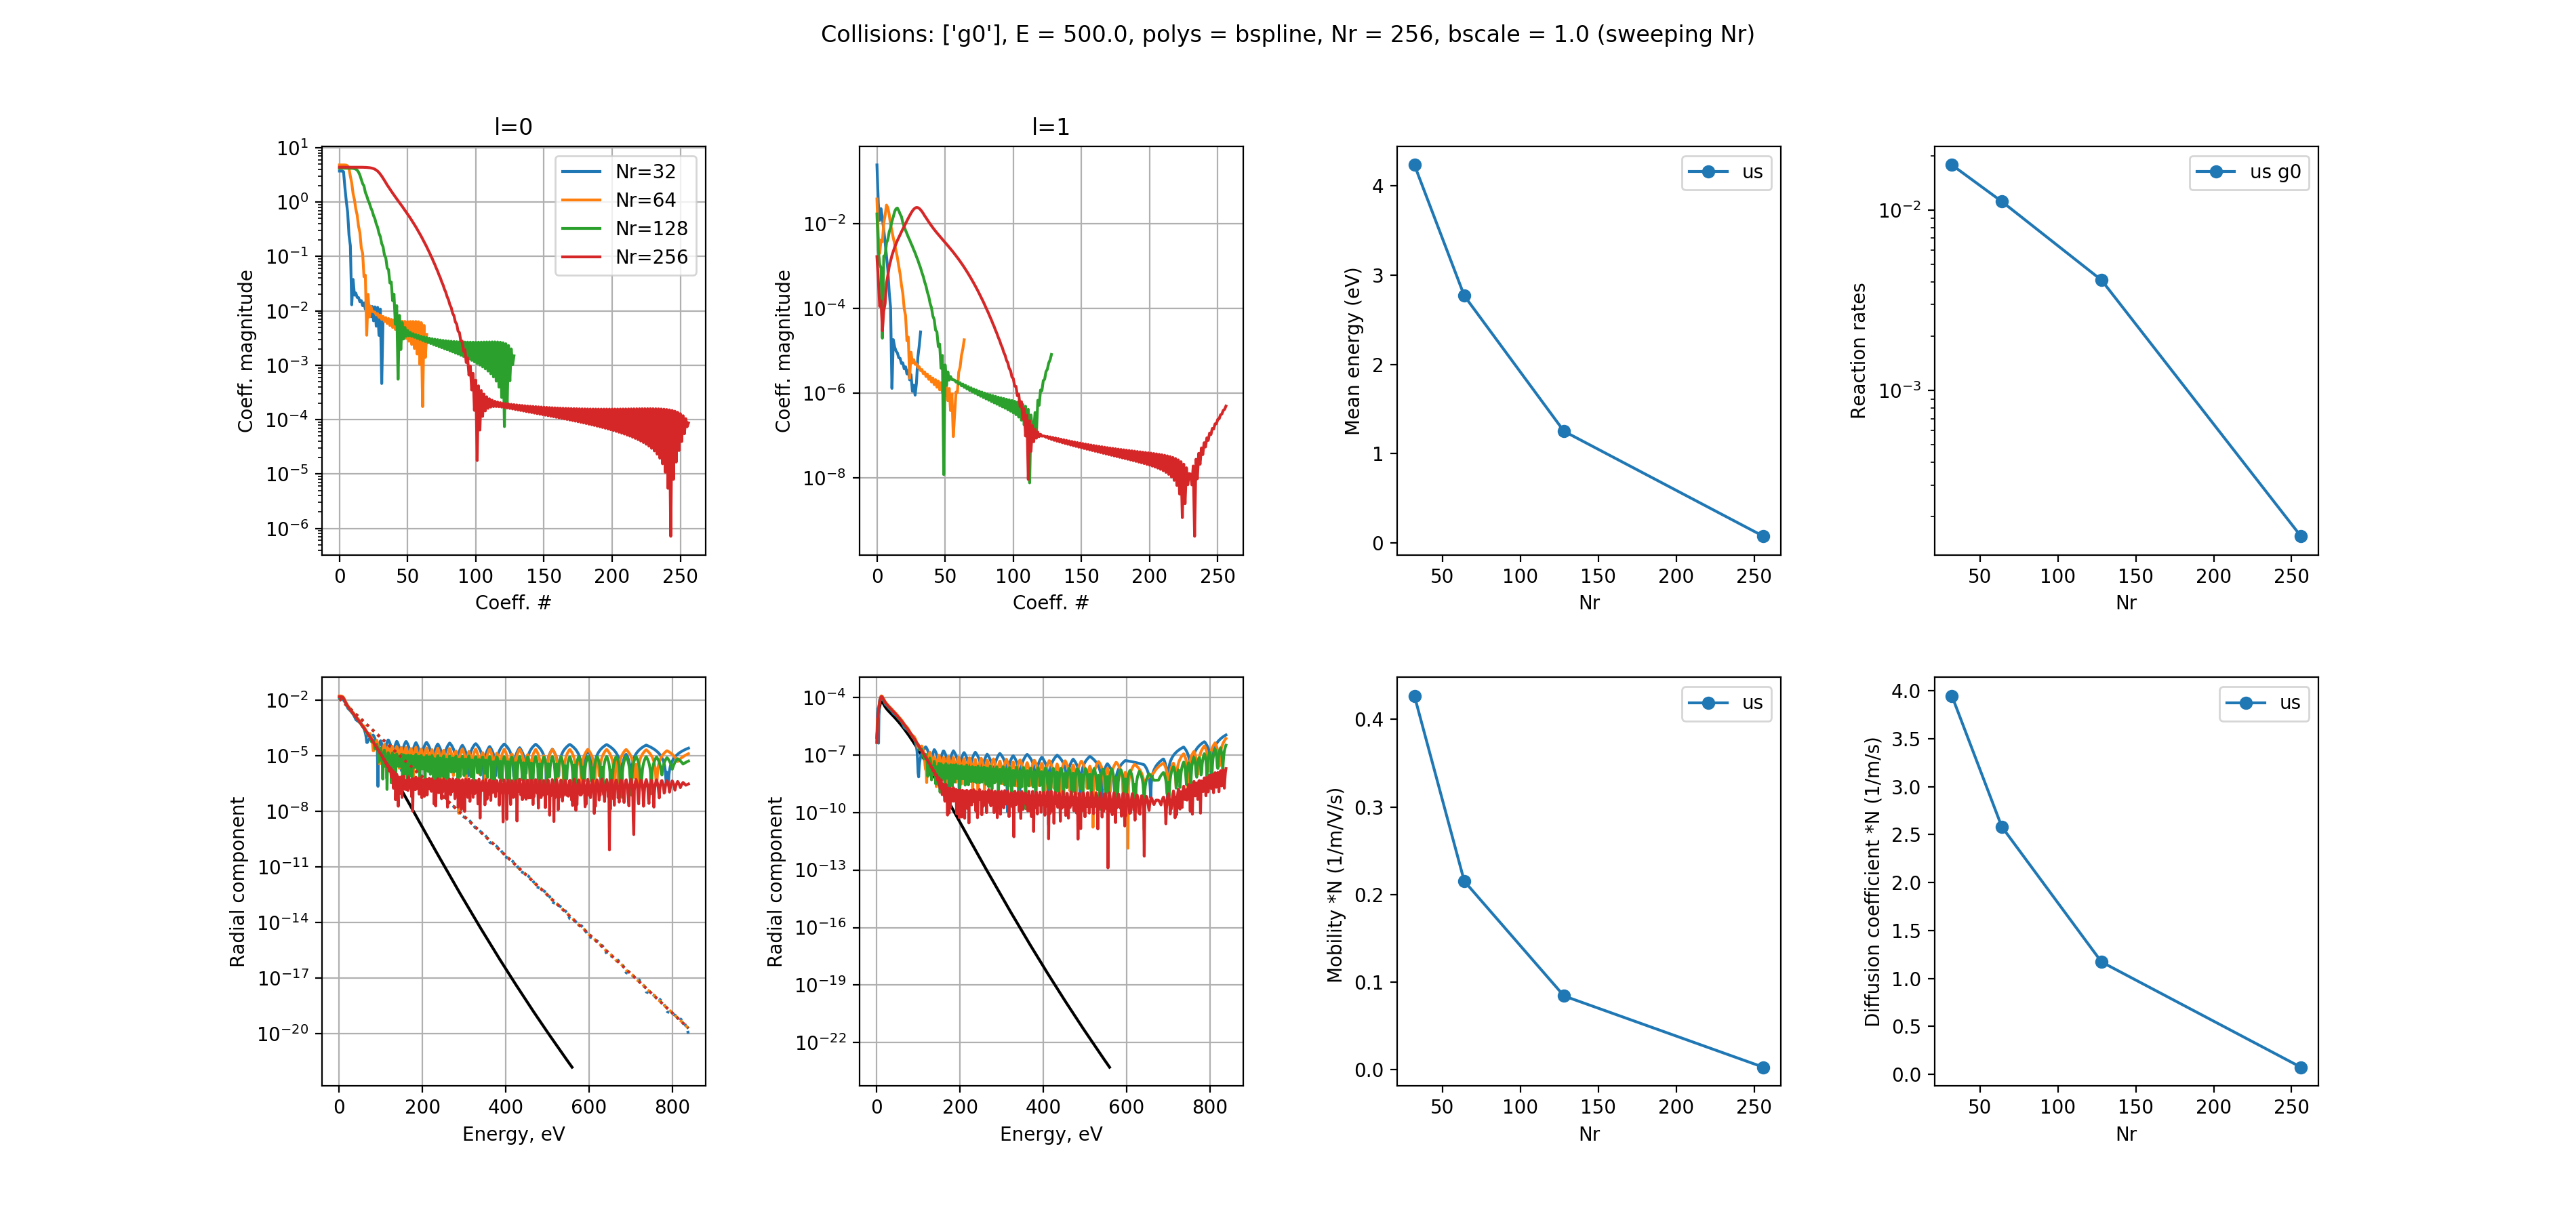
\includegraphics[width=\textwidth]{figures/maxwell_vs_bolsig_g0_E500.0_poly_bspline_nr256_bscale1.0_sweeping_Nr.png}}
	\end{center}
\end{frame}

\begin{frame}
	\begin{itemize}
		\item With elastic + ionization collisions with increasing $\vect{E}$ (curve-fitted cross sections to LXCAT).
	\end{itemize}
	\begin{center}
		\only<+>{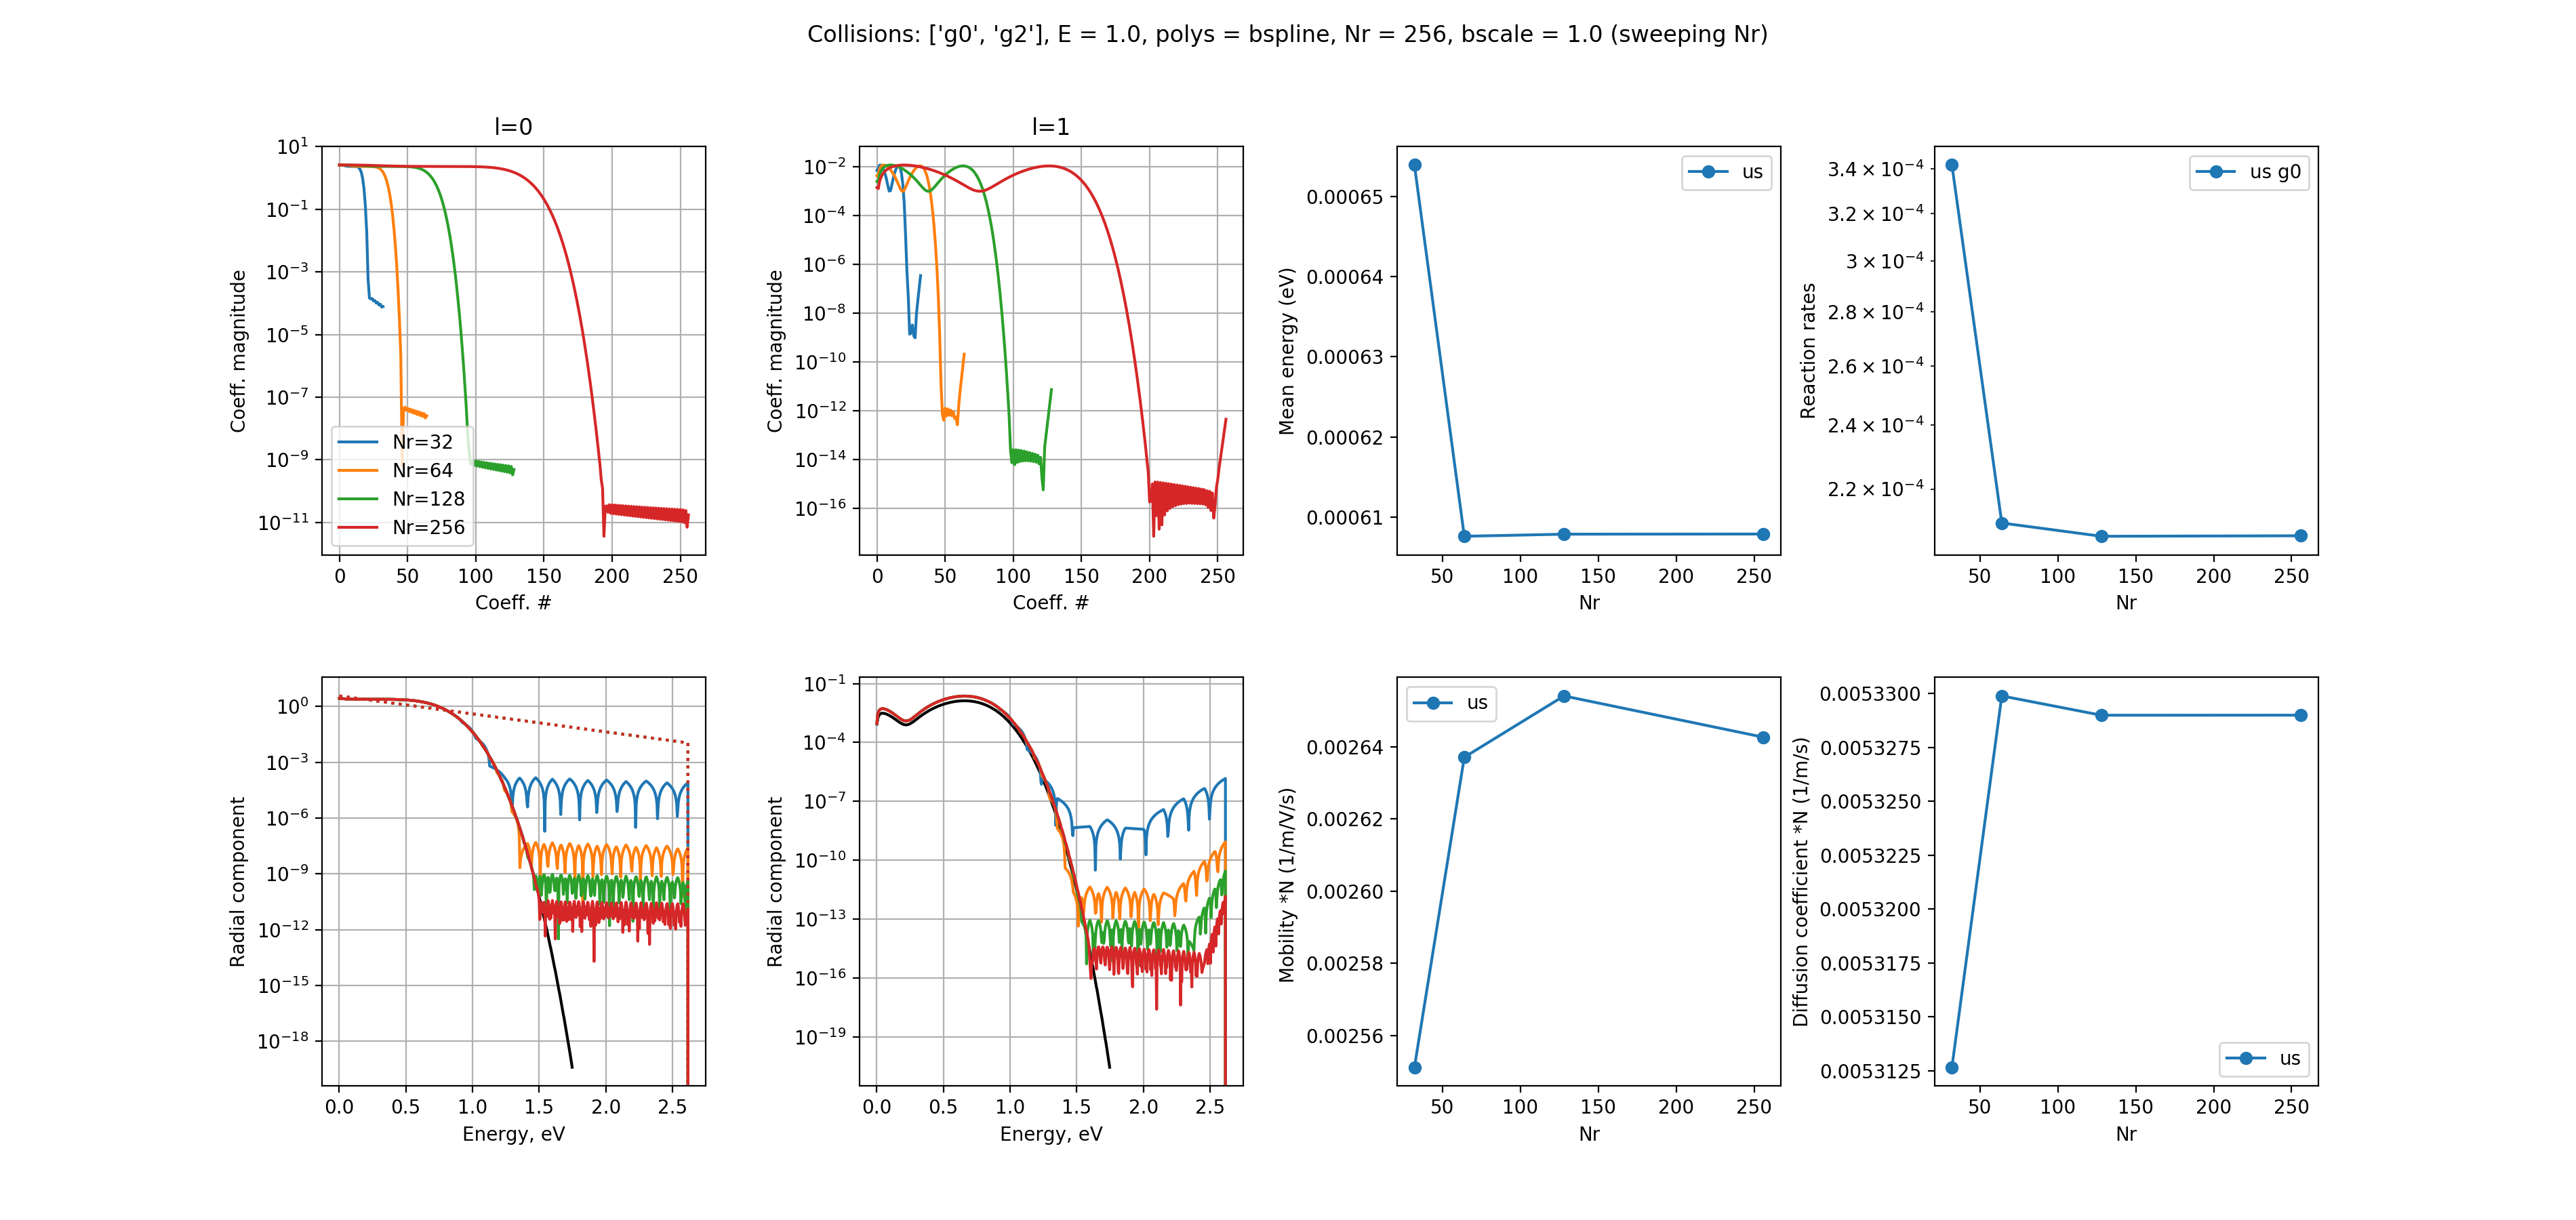
\includegraphics[width=\textwidth]{figures/maxwell_vs_bolsig_g0_g2_E1.0_poly_bspline_nr256_bscale1.0_sweeping_Nr.png}}
		\only<+>{\includegraphics[width=\textwidth]{figures/maxwell_vs_bolsig_g0_g2_E10.0_poly_bspline_nr256_bscale1.0_sweeping_Nr.png}}
		\only<+>{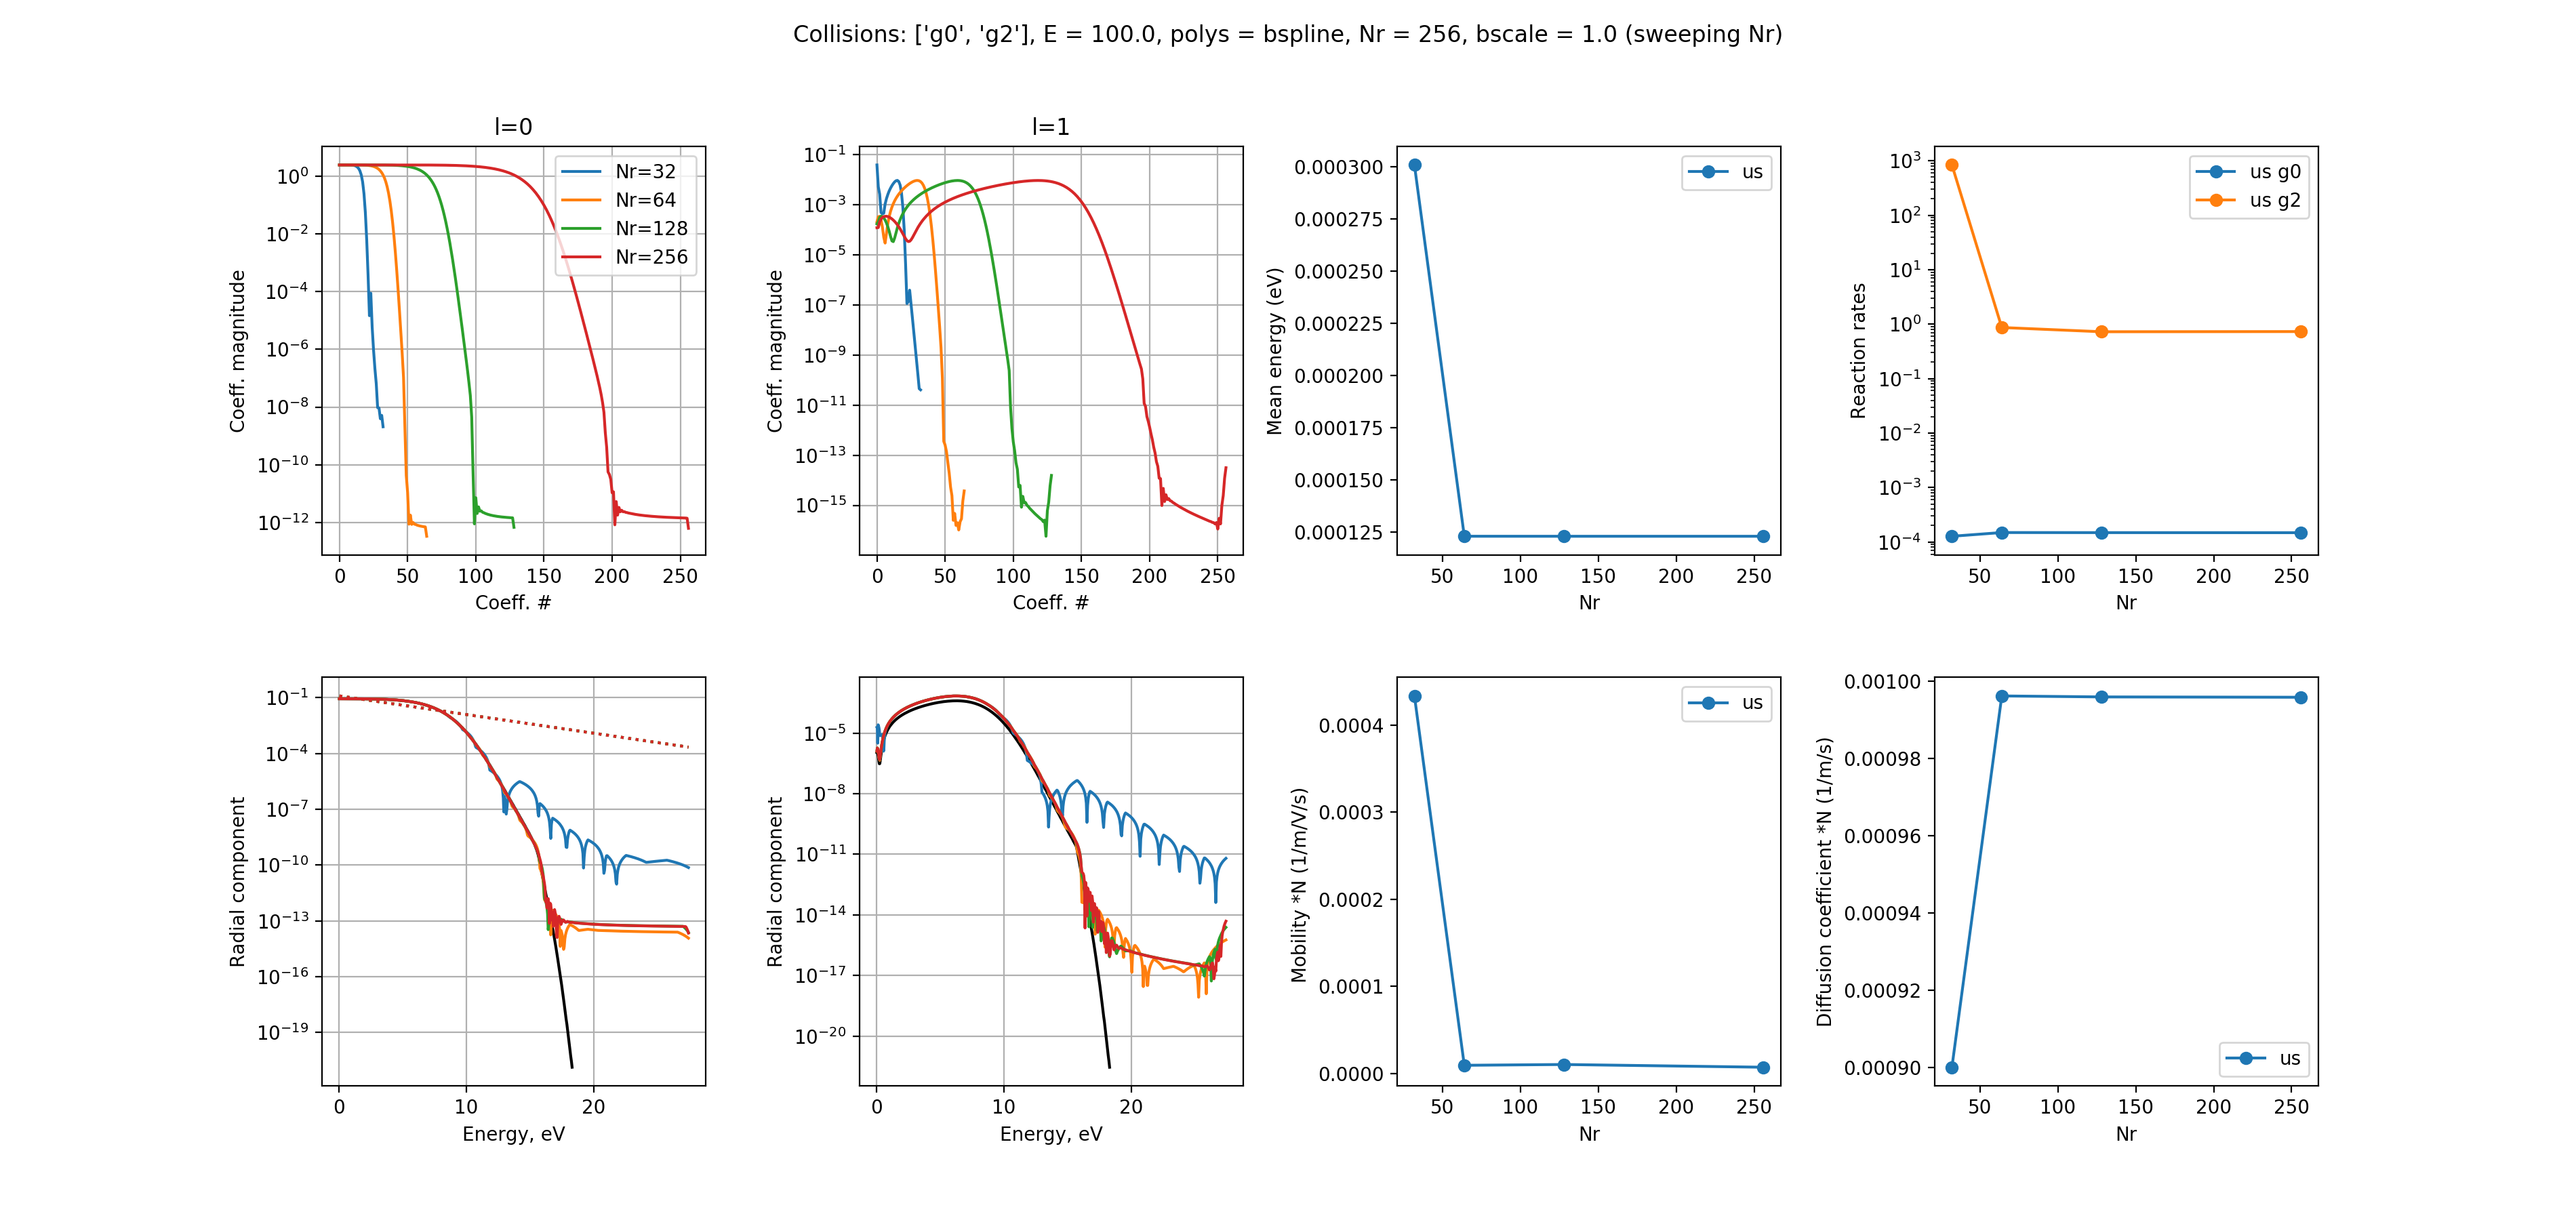
\includegraphics[width=\textwidth]{figures/maxwell_vs_bolsig_g0_g2_E100.0_poly_bspline_nr256_bscale1.0_sweeping_Nr.png}}
		\only<+>{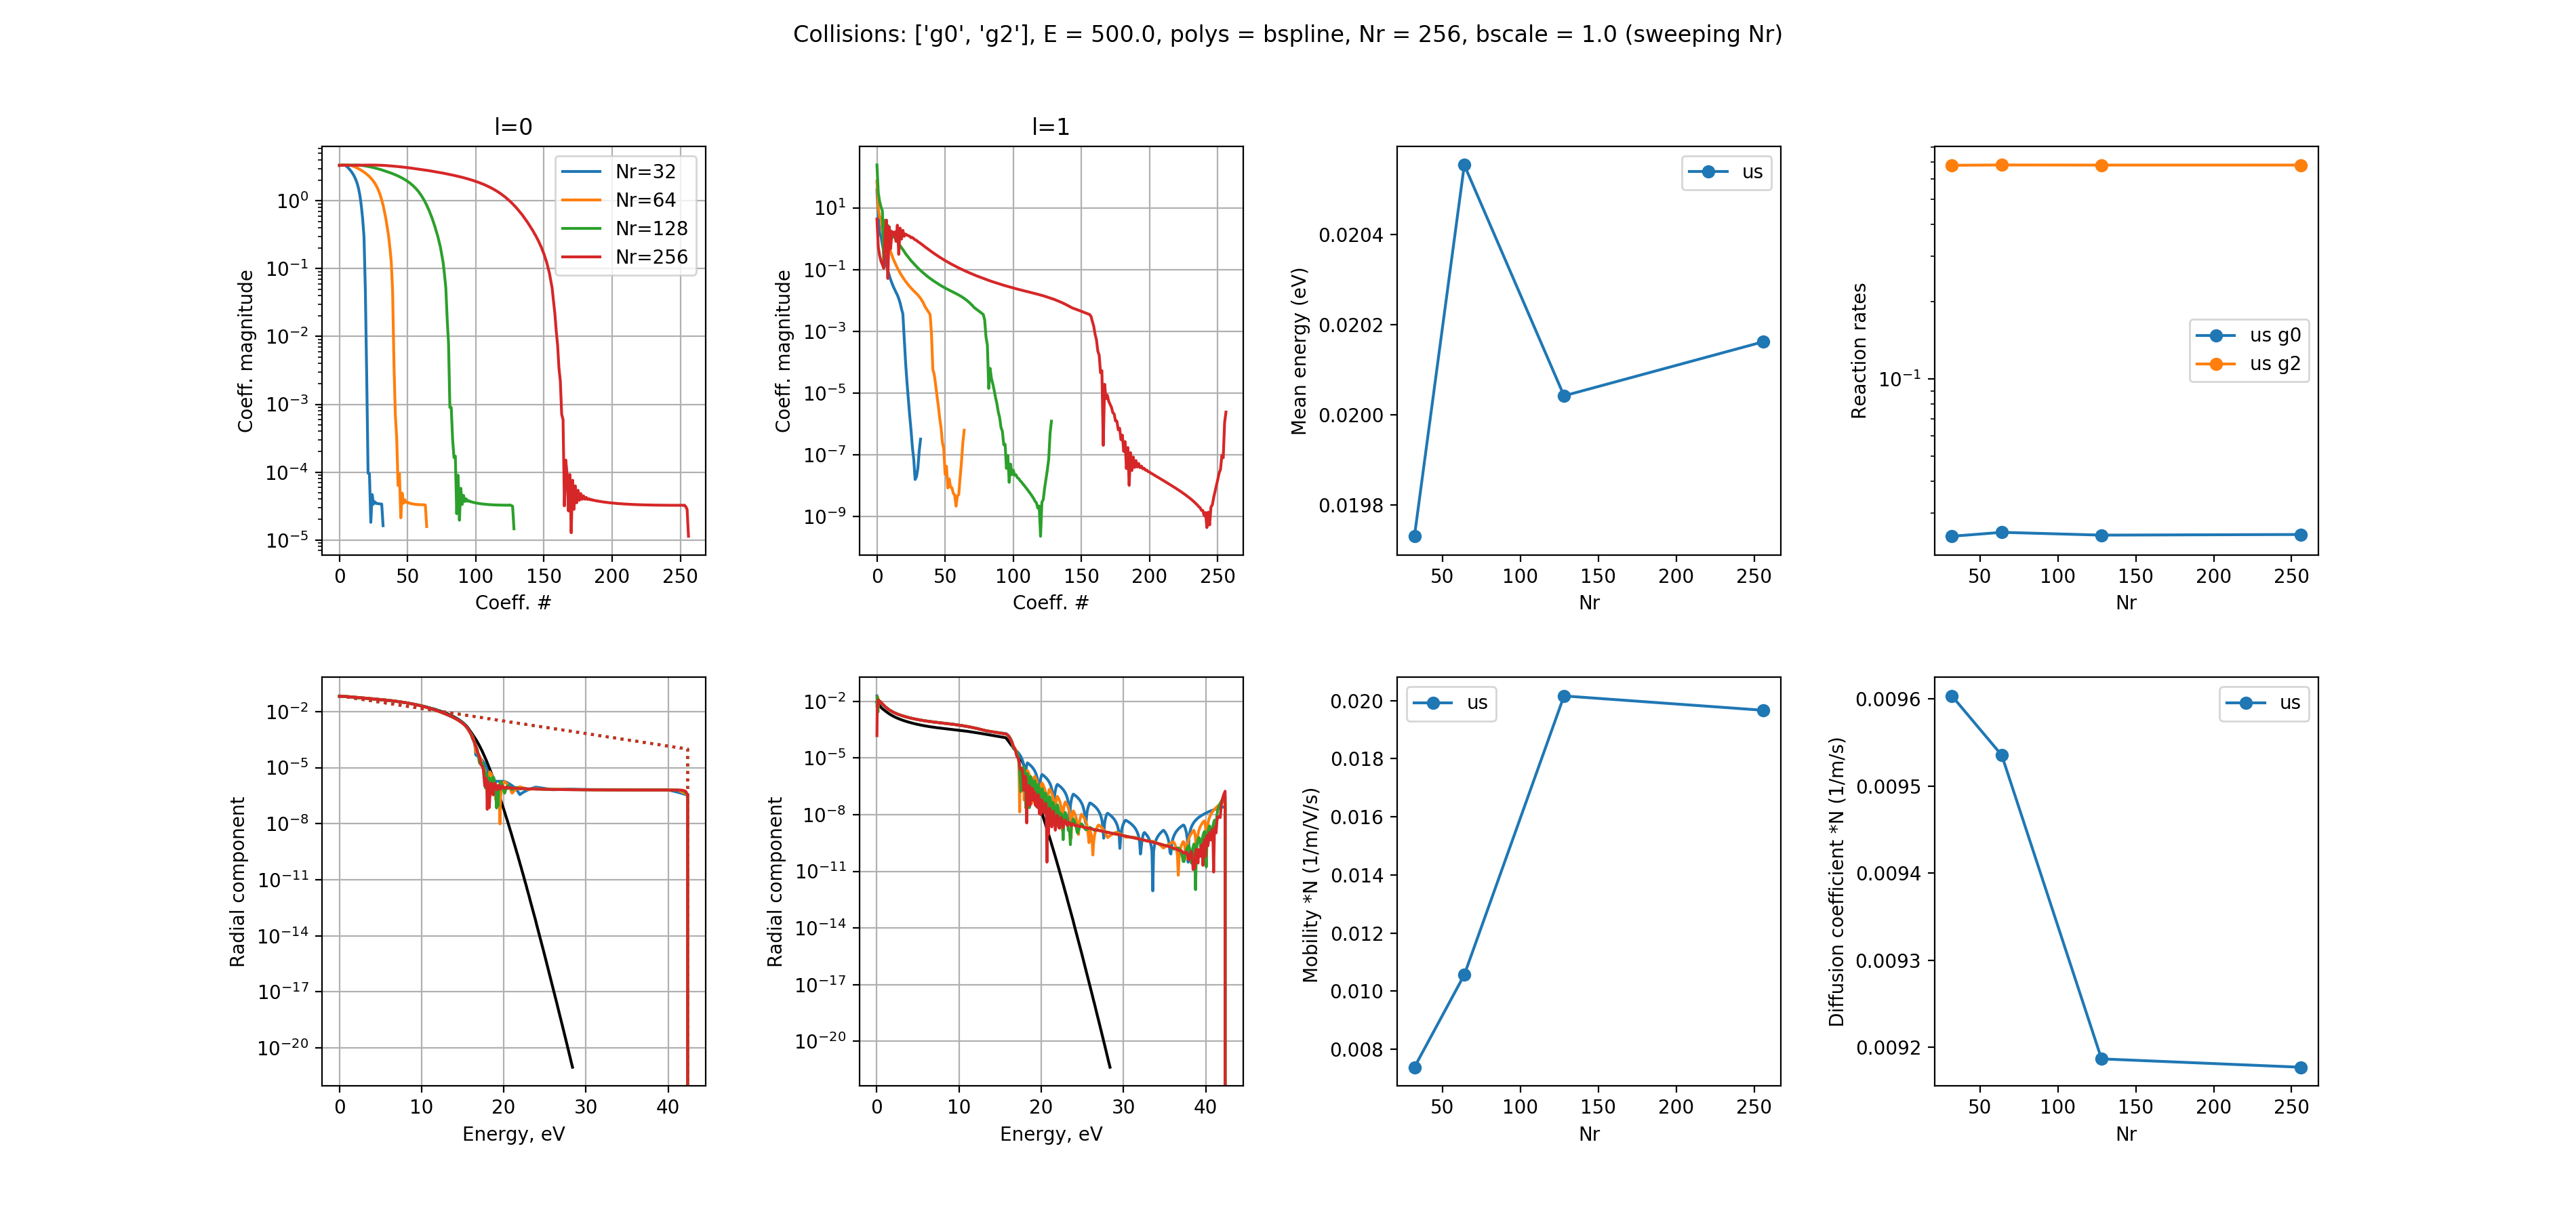
\includegraphics[width=\textwidth]{figures/maxwell_vs_bolsig_g0_g2_E500.0_poly_bspline_nr256_bscale1.0_sweeping_Nr.png}}
		\only<+>{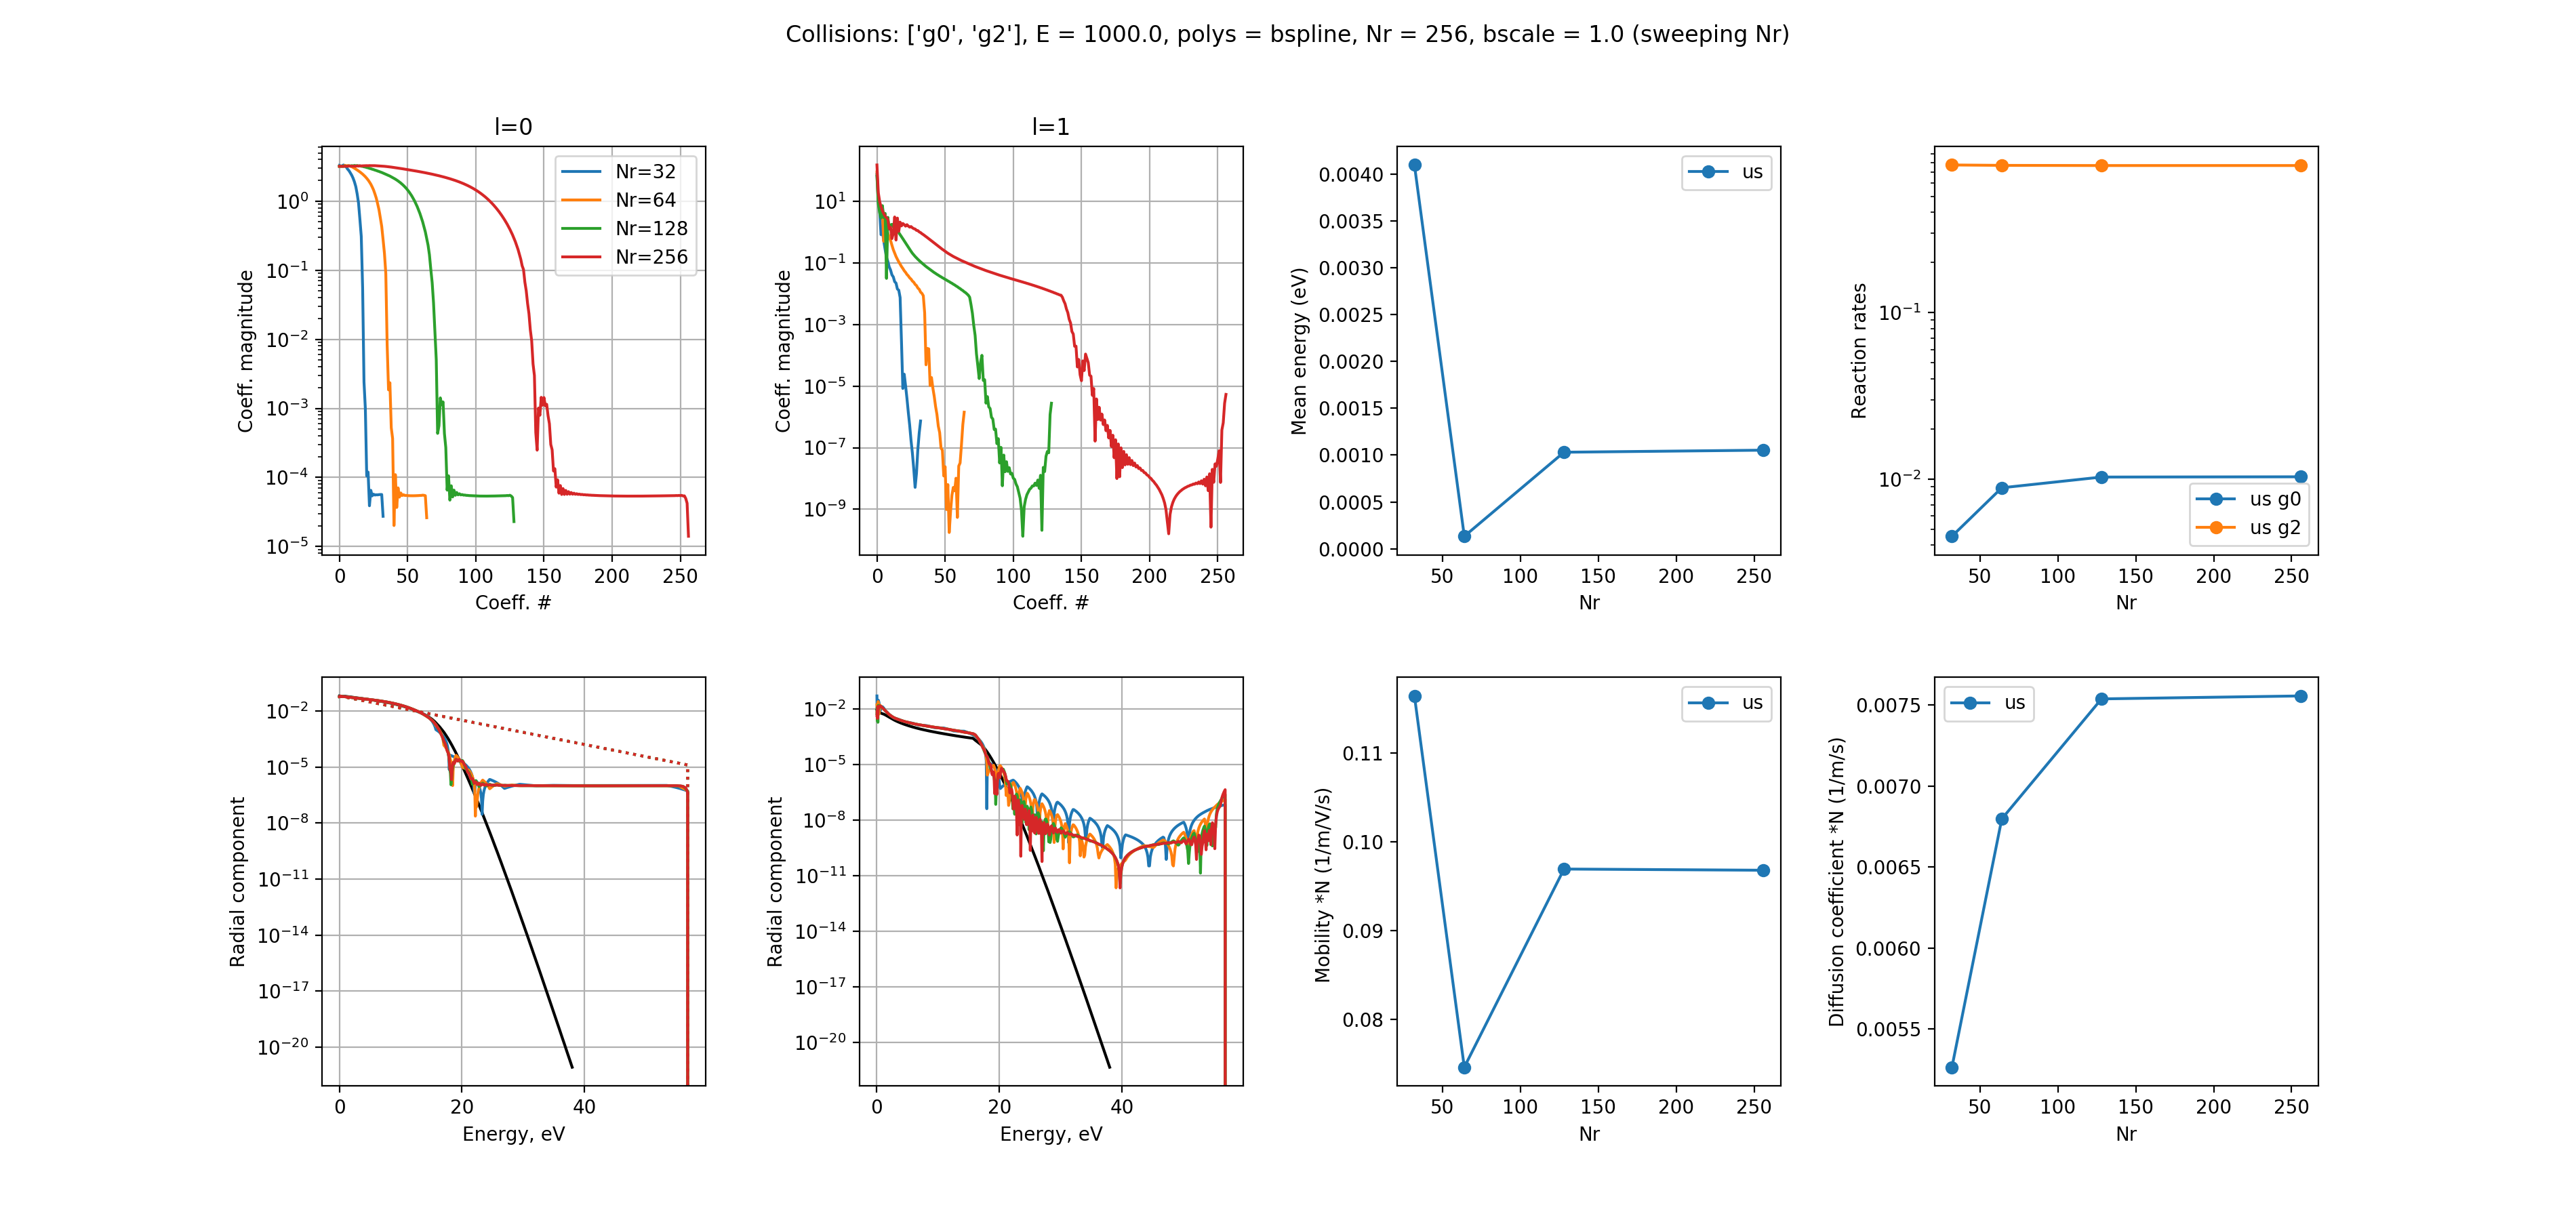
\includegraphics[width=\textwidth]{figures/maxwell_vs_bolsig_g0_g2_E1000.0_poly_bspline_nr256_bscale1.0_sweeping_Nr.png}}
		\only<+>{\includegraphics[width=\textwidth]{figures/maxwell_vs_bolsig_g0_g2_E5000.0_poly_bspline_nr256_bscale1.0_sweeping_Nr.png}}
	\end{center}
\end{frame}






%===============================================================================
\end{document}

